%%%%%%%%%%%%%%
%% Run LaTeX on this file several times to get Table of Contents,
%% cross-references, and citations.

%% If you have font problems, you may edit the w-bookps.sty file
%% to customize the font names to match those on your system.

%% w-bksamp.tex. Current Version: Feb 16, 2012
%%%%%%%%%%%%%%%%%%%%%%%%%%%%%%%%%%%%%%%%%%%%%%%%%%%%%%%%%%%%%%%%
%
%  Sample file for
%  Wiley Book Style, Design No.: SD 001B, 7x10
%  Wiley Book Style, Design No.: SD 004B, 6x9
%
%
%  Prepared by Amy Hendrickson, TeXnology Inc.
%  http://www.texnology.com
%%%%%%%%%%%%%%%%%%%%%%%%%%%%%%%%%%%%%%%%%%%%%%%%%%%%%%%%%%%%%%%%

%%%%%%%%%%%%%
% 7x10
%\documentclass{wileySev}

% 6x9
\documentclass{wileysix}

\usepackage{graphicx}
\usepackage{listings}
\usepackage{float}
\usepackage{color}
 
\definecolor{codegreen}{rgb}{0,0.6,0}
\definecolor{codegray}{rgb}{0.5,0.5,0.5}
\definecolor{codepurple}{rgb}{0.58,0,0.82}
\definecolor{backcolour}{rgb}{0.95,0.95,0.92}
 
\lstdefinestyle{mystyle}{
    backgroundcolor=\color{backcolour},   
    commentstyle=\color{codegreen},
    keywordstyle=\color{magenta},
    numberstyle=\tiny\color{codegray},
    stringstyle=\color{codepurple},
    basicstyle=\footnotesize,
    breakatwhitespace=false,         
    breaklines=true,                 
    captionpos=b,                    
    keepspaces=true,                 
    numbers=left,                    
    numbersep=5pt,                  
    showspaces=false,                
    showstringspaces=false,
    showtabs=false,                  
    tabsize=2,
    language=sh
}
 
\lstset{style=mystyle}

%%%%%%%
%% for times math: However, this package disables bold math (!)
%% \mathbf{x} will still work, but you will not have bold math
%% in section heads or chapter titles. If you don't use math
%% in those environments, mathptmx might be a good choice.

% \usepackage{mathptmx}

% For PostScript text
\usepackage{w-bookps}

%%%%%%%%%%%%%%%%%%%%%%%%%%%%%%%%%%%%%%%%%%%%%%%%%%%%%%%%%%%%%%%%
%% Other packages you might want to use:

% for chapter bibliography made with BibTeX
% \usepackage{chapterbib}

% for multiple indices
% \usepackage{multind}

% for answers to problems
% \usepackage{answers}

%%%%%%%%%%%%%%%%%%%%%%%%%%%%%%
%% Change options here if you want:
%%
%% How many levels of section head would you like numbered?
%% 0= no section numbers, 1= section, 2= subsection, 3= subsubsection
%%==>>
\setcounter{secnumdepth}{3}

%% How many levels of section head would you like to appear in the
%% Table of Contents?
%% 0= chapter titles, 1= section titles, 2= subsection titles, 
%% 3= subsubsection titles.
%%==>>
\setcounter{tocdepth}{2}

%% Cropmarks? good for final page makeup
%% \docropmarks

%%%%%%%%%%%%%%%%%%%%%%%%%%%%%%
%
% DRAFT
%
% Uncomment to get double spacing between lines, current date and time
% printed at bottom of page.
% \draft
% (If you want to keep tables from becoming double spaced also uncomment
% this):
% \renewcommand{\arraystretch}{0.6}
%%%%%%%%%%%%%%%%%%%%%%%%%%%%%%

%%%%%%% Demo of section head containing sample macro:
%% To get a macro to expand correctly in a section head, with upper and
%% lower case math, put the definition and set the box 
%% before \begin{document}, so that when it appears in the 
%% table of contents it will also work:

\newcommand{\VT}[1]{\ensuremath{{V_{T#1}}}}

%% use a box to expand the macro before we put it into the section head:

\newbox\sectsavebox
\setbox\sectsavebox=\hbox{\boldmath\VT{xyz}}

%%%%%%%%%%%%%%%%% End Demo


\begin{document}


\booktitle{Tutorial Android}
\subtitle{Membuat Aplikasi Monitoring Kinerja Berbasis GPS}


\authors{M. Yusril H. S., Kadek Diva K. M., \& Chandra Kirana Poetra\\
\affil{Politeknik Pos Indonesia}
%Floyd J. Fowler, Jr.\\
%\affil{University of New Mexico}
}

\offprintinfo{Tutorial Android, First Edition}{M. Yusril H. S., Kadek Diva K. M., \& Chandra Kirana P.}

%% Can use \\ if title, and edition are too wide, ie,
%% \offprintinfo{Survey Methodology,\\ Second Edition}{Robert M. Groves}

%%%%%%%%%%%%%%%%%%%%%%%%%%%%%%
%% 
\halftitlepage

\titlepage


\begin{copyrightpage}{2020}
%Survey Methodology / Robert M. Groves . . . [et al.].
%\       p. cm.---(Wiley series in survey methodology)
%\    ``Wiley-Interscience."
%\    Includes bibliographical references and index.
%\    ISBN 0-471-48348-6 (pbk.)
%\    1. Surveys---Methodology.  2. Social 
%\  sciences---Research---Statistical methods.  I. Groves, Robert M.  II. %
%Series.\\
%
%HA31.2.S873 2007
%001.4'33---dc22                                             2004044064
\end{copyrightpage}

\begin{preface}
	Buku ini diciptakan bagi yang awam dengan pemrograman android sekalipun.

\prefaceauthor{R. M. Awangga}
\where{Bandung, Jawa Barat\\
Februari, 2019}
\end{preface}

%\dedication{`Jika Kamu tidak dapat menahan lelahnya belajar, 
%Maka kamu harus sanggup menahan perihnya Kebodohan.'
%~Imam Syafi'i~}

%\begin{contributors}
%\name{Rolly Maulana Awangga,} Informatics Research Center., Politeknik Pos Indonesia, Bandung,
Indonesia



%\end{contributors}

%\contentsinbrief
\tableofcontents
\listoffigures
%\listoftables
%\lstlistoflistings


\begin{foreword}
Sepatah kata dari Kaprodi, Kabag Kemahasiswaan dan Mahasiswa
\end{foreword}



\begin{acknowledgments}
Terima kasih atas semua masukan dari para mahasiswa agar bisa membuat buku ini 
lebih baik dan lebih mudah dimengerti.

Terima kasih ini juga ditujukan khusus untuk team IRC yang 
telah fokus untuk belajar dan memahami bagaimana buku ini mendampingi proses 
Intership.
\authorinitials{R. M. A.}
\end{acknowledgments}

\begin{acronyms}
\acro{ACGIH}{American Conference of Governmental Industrial Hygienists}
\acro{AEC}{Atomic Energy Commission}
\acro{OSHA}{Occupational Health and Safety Commission}
\acro{SAMA}{Scientific Apparatus Makers Association}
\end{acronyms}

\begin{glossary}
\term{git}Merupakan manajemen sumber kode yang dibuat oleh linus torvald.

\term{bash}Merupakan bahasa sistem operasi berbasiskan *NIX.

\term{linux}Sistem operasi berbasis sumber kode terbuka yang dibuat oleh Linus Torvald
\end{glossary}

%\begin{symbols}
%\term{A}Amplitude

\term{\hbox{\&}}Propositional logic symbol 

\term{a}Filter Coefficient

\bigskip

\term{\mathcal{B}}Number of Beats
%\end{symbols}

\begin{introduction}

%% optional, but if you want to list author:

\introauthor{Rolly Maulana Awangga, S.T., M.T.}
{Informatics Research Center\\
Bandung, Jawa Barat, Indonesia}

Pada era disruptif  \index{disruptif}\index{disruptif!modern} 
saat ini. git merupakan sebuah kebutuhan dalam sebuah organisasi pengembangan perangkat lunak.
Buku ini diharapkan bisa menjadi penghantar para programmer, analis, IT Operation dan Project Manajer.
Dalam melakukan implementasi git pada diri dan organisasinya.

Rumusnya cuman sebagai contoh aja biar keren\cite{awangga2018sampeu}.

\begin{equation}
ABC {\cal DEF} \alpha\beta\Gamma\Delta\sum^{abc}_{def}
\end{equation}

\end{introduction}

%%%%%%%%%%%%%%%%%%Isi Buku_

\chapter{Chapter 1}
\section{1174004 - Choirulanam}
\subsection{Data Types}
	\hfill\break
	Tipe data Struktur paling signifikan dalam Python adalah list, tupel, dan dictionary. Set telah diintegrasikan ke dalam Python sejak versi 2.5 (versi sebelumnya tersedia di perpustakaan set): List: Ini mirip dengan array satu dimensi, tetapi Anda dapat membuat daftar yang berisi daftar lain. Dictionary: Ini adalah array yang berisi pasangan kunci dan nilai-nilai (tabel hash). Tuples: Ini adalah objek mono-dimensi abadi. Array dapat berupa jenis apa saja, sehingga Anda dapat mencampur variabel seperti bilangan bulat dan string ke dalam daftar, kamus, dan tupel Anda. Indeks objek pertama dalam semua jenis array selalu nol. Indeks negatif diizinkan dan dihitung dari akhir array; -1 menunjukkan elemen terakhir dari array:

	\begin{itemize}
		\item Contoh List
		\hfill\break
	           \lstinputlisting[firstline=7, lastline=11]{src/kelompok1/srcsistemtersebar.py}
		\hfill\break
		dan berikut hasilnya:
		\begin{figure}[H]
		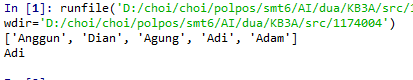
\includegraphics[width=4cm]{figures/kelompok1/1/anam/list.png}
		\centering
		\caption{List}
		\end{figure}

		\item Contoh Dictionary
		\hfill\break
	           \lstinputlisting[firstline=13, lastline=17]{src/kelompok1/srcsistemtersebar.py}
		\hfill\break
		dan berikut hasilnya:
		\begin{figure}[H]
		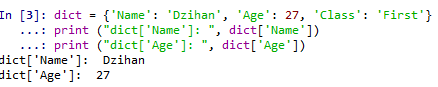
\includegraphics[width=4cm]{figures/kelompok1/1/anam/dict.png}
		\centering
		\caption{Dictionary}
		\end{figure}

		\item Contoh Tuple
		\hfill\break
	           \lstinputlisting[firstline=19, lastline=25]{src/kelompok1/srcsistemtersebar.py}
		\hfill\break
		dan berikut hasilnya:
		\begin{figure}[H]
		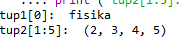
\includegraphics[width=4cm]{figures/kelompok1/1/anam/tupl.png}
		\centering
		\caption{Tuple}
		\end{figure}
	\end{itemize}

\subsection{String}
	\hfill\break
	String python diindikasikan menggunakan tanda kutip tunggal (') atau ganda (") dan diizinkan menggunakan satu notasi dalam string yang dibatasi oleh yang lain:
	\begin{itemize}
		\item Contoh String
		\hfill\break
	           \lstinputlisting[firstline=27, lastline=34]{src/kelompok1/srcsistemtersebar.py}
		\hfill\break
		dan berikut hasilnya:
		\begin{figure}[H]
		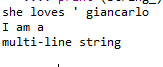
\includegraphics[width=4cm]{figures/kelompok1/1/anam/string.png}
		\centering
		\caption{String}
		\end{figure}
	\end{itemize}

\subsection{Bukti Tidak Plagiat}
\begin{figure}[H]
	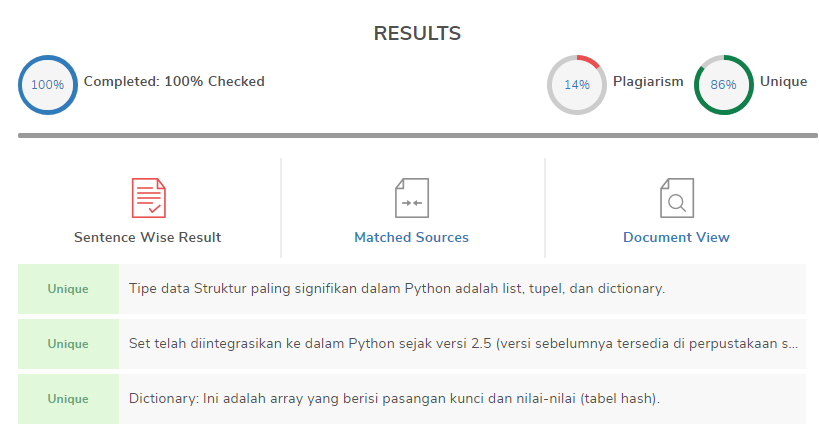
\includegraphics[width=4cm]{figures/kelompok1/1/anam/plagiat_anam.png}
	\centering
	\caption{Bukti Tidak Melakukan Plagiat Chapter 1}
\end{figure}

\section{1174012 - Damara Benedikta}
\subsection{Flow control }
Flow control merupakan sebuah pengelolaan (data flow) atau aliran data antara komputer atau perangkat atau antar node dalam suatu jaringan sehingga data dapat ditangani dengan kecepatan yang efisien.
Dimana terdapat if, for dan while. Terdapat dua jenis perualangan dalam bahasa pemrograman python, yaitu perulangan dengan for dan while
Perulangan for disebut counted loop (perulangan yang terhitung), sementara perulangan while disebut uncounted loop (perulangan yang tak terhitung). Perbedaannya adalah perulangan for biasanya digunakan untuk mengulangi kode yang sudah diketahui banyak perulangannya. Sementara while untuk perulangan yang memiliki syarat dan tidak tentu berapa banyak perulangannya.
Serta Kondisi If Pengambilan keputusan (kondisi if) digunakan untuk mengantisipasi kondisi yang terjadi saat jalanya program dan menentukan tindakan apa yang akan diambil sesuai dengan kondisi.
\hfill\break
\lstinputlisting[firstline=8, lastline=21]{src/kelompok1/perulangan.py}
\hfill\break

	\begin{figure}[H]
		\centering
		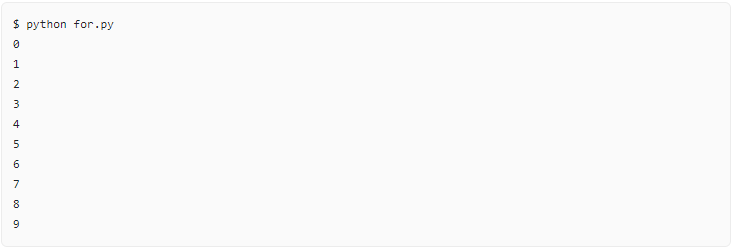
\includegraphics[width=4cm]{figures/kelompok1/1/damara/o_for.PNG}
		\caption{contoh perulangan for}
	\end{figure}

	\begin{figure}[H]
		\centering
		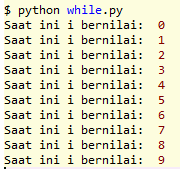
\includegraphics[width=4cm]{figures/kelompok1/1/damara/o_while.PNG}
		\caption{contoh perulangan while}
	\end{figure}

\subsection{Functions}
Fungsi adalah bagian dari program yang dapat digunakan ulang. Hal ini bisa dicapai dengan memberi nama pada blok statemen, kemudian nama ini dapat dipanggil di manapun dalam program. Kita telah menggunakan beberapa fungsi builtin seperti range.
Fungsi dalam Python didefinisikan menggunakan kata kunci def. Setelah def ada nama pengenal fungsi diikut dengan parameter yang diapit oleh tanda kurung dan diakhir dingan tanda titik dua 
\hfill\break
\lstinputlisting[firstline=23, lastline=44]{src/kelompok1/perulangan.py}
\hfill\break
\subsection{Bukti Tidak Plagiat}
\begin{figure}[H]
\centering
	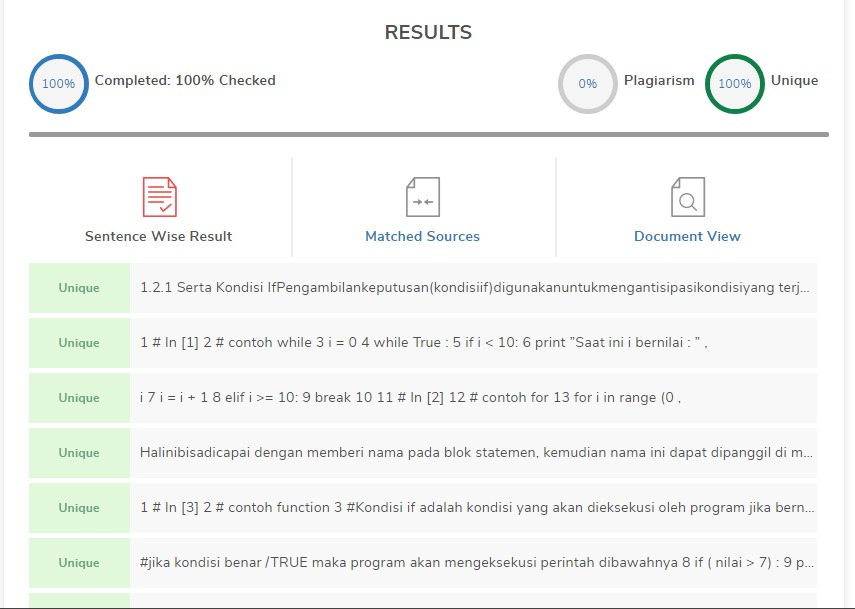
\includegraphics[width=4cm]{figures/kelompok1/1/damara/plagiat.jpeg}
	\caption{Bukti Tidak Melakukan Plagiat Chapter 1}
\end{figure}

\section{1174095 - Muhammad Dzihan}
\subsection{Class}
Python mendukung banyak warisan kelas. Secara konvensional (bukan aturan bahasa), variabel dan metode pribadi dideklarasikan dengan didahului dengan dua garis bawah. Kita dapat menetapkan atribut (properti) yang berubah-ubah ke instance kelas, seperti yang ditunjukkan pada contoh berikut:
\hfill\break
\lstinputlisting[firstline=7, lastline=16]{src/kelompok1/class.py}

\hfill\break
	\begin{figure}[H]
		\centering
		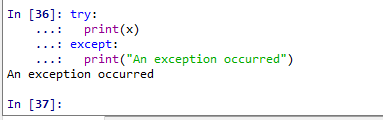
\includegraphics[width=4cm]{figures/kelompok1/1/dzihan/class1.PNG}
		\caption{Exceptions1}
	\end{figure}
\hfill\break
\lstinputlisting[firstline=17, lastline=20]{src/kelompok1/class.py}

\hfill\break
	\begin{figure}[H]
		\centering
		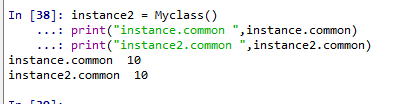
\includegraphics[width=4cm]{figures/kelompok1/1/dzihan/class2.PNG}
		\caption{Exceptions2}
	\end{figure}
\hfill\break
\lstinputlisting[firstline=21, lastline=26]{src/kelompok1/class.py}

\hfill\break
	\begin{figure}[H]
		\centering
		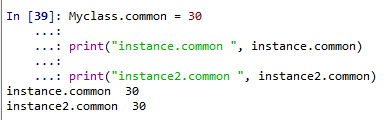
\includegraphics[width=4cm]{figures/kelompok1/1/dzihan/class3.PNG}
		\caption{Exceptions3}
	\end{figure}
\hfill\break
\lstinputlisting[firstline=27, lastline=31]{src/kelompok1/class.py}

\hfill\break
	\begin{figure}[H]
		\centering
		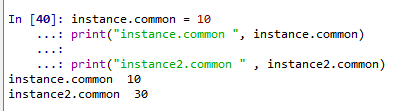
\includegraphics[width=4cm]{figures/kelompok1/1/dzihan/class4.PNG}
		\caption{Exceptions4}
	\end{figure}
\hfill\break
\lstinputlisting[firstline=32, lastline=36]{src/kelompok1/class.py}

\hfill\break
	\begin{figure}[H]
		\centering
		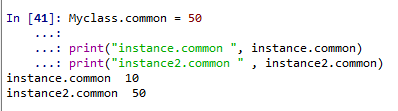
\includegraphics[width=4cm]{figures/kelompok1/1/dzihan/class5.PNG}
		\caption{Exceptions5}
	\end{figure}
\hfill\break
\lstinputlisting[firstline=37, lastline=47]{src/kelompok1/class.py}

\hfill\break
	\begin{figure}[H]
		\centering
		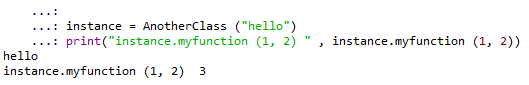
\includegraphics[width=4cm]{figures/kelompok1/1/dzihan/class6.PNG}
		\caption{Exceptions6}
	\end{figure}
\hfill\break
\lstinputlisting[firstline=48, lastline=51]{src/kelompok1/class.py}

\hfill\break
	\begin{figure}[H]
		\centering
		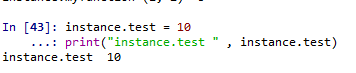
\includegraphics[width=4cm]{figures/kelompok1/1/dzihan/class7.PNG}
		\caption{Exceptions7}
	\end{figure}
\subsection{Exceptions}
Exceptions adalah peristiwa yang terjadi selama pelaksanaan program yang mengganggu aliran normal instruksi program. Secara umum, ketika skrip Python menemukan situasi yang tidak dapat diatasi, itu menimbulkan pengecualian. Pengecualian adalah objek Python yang mewakili kesalahan.
\hfill\break
\lstinputlisting[firstline=7, lastline=11]{src/kelompok1/exception.py}
\hfill\break
	\begin{figure}[H]
		\centering
		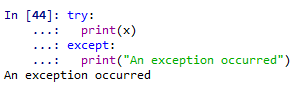
\includegraphics[width=4cm]{figures/kelompok1/1/dzihan/exc1.PNG}
		\caption{Exceptions1}
	\end{figure}
\hfill\break
\lstinputlisting[firstline=12, lastline=18]{src/kelompok1/exception.py}
\hfill\break
	\begin{figure}[H]
		\centering
		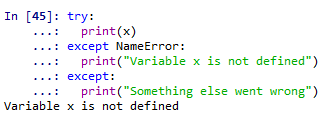
\includegraphics[width=4cm]{figures/kelompok1/1/dzihan/exc2.PNG}
		\caption{Exceptions2}
	\end{figure}
\hfill\break
\lstinputlisting[firstline=19, lastline=25]{src/kelompok1/exception.py}
\hfill\break
	\begin{figure}[H]
		\centering
		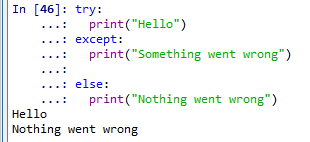
\includegraphics[width=4cm]{figures/kelompok1/1/dzihan/exc3.PNG}
		\caption{Exceptions3}
	\end{figure}
\hfill\break
\lstinputlisting[firstline=26, lastline=32]{src/kelompok1/exception.py}
\hfill\break
	\begin{figure}[H]
		\centering
		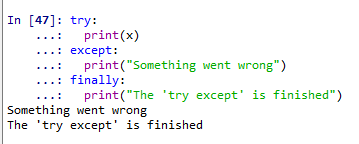
\includegraphics[width=4cm]{figures/kelompok1/1/dzihan/exc4.PNG}
		\caption{Exceptions4}
	\end{figure}
\hfill\break
\lstinputlisting[firstline=33, lastline=40]{src/kelompok1/exception.py}
\hfill\break
	\begin{figure}[H]
		\centering
		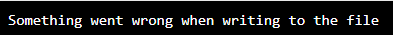
\includegraphics[width=4cm]{figures/kelompok1/1/dzihan/exc5.PNG}
		\caption{Exceptions5}
	\end{figure}

\subsection{Bukti Tidak Plagiat}
\begin{figure}[H]
\centering
	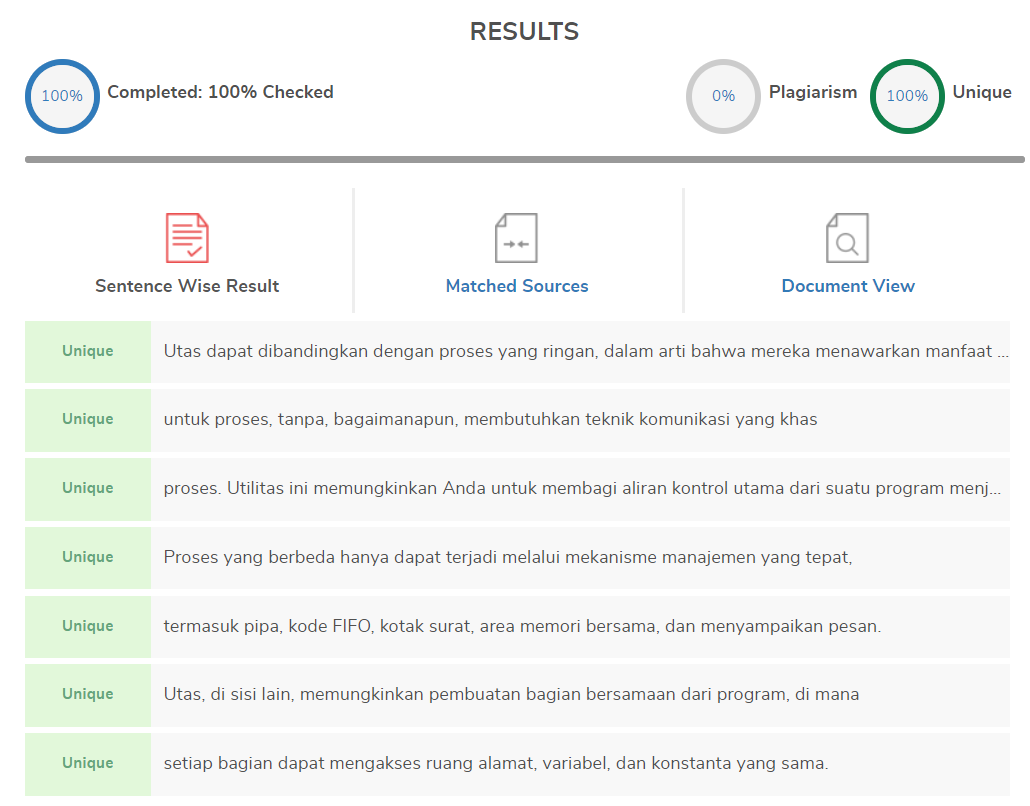
\includegraphics[width=4cm]{figures/kelompok1/1/dzihan/plagiat.PNG}
	\caption{Bukti Tidak Melakukan Plagiat Chapter 1}
\end{figure}


\section{1174021 - Muhammad Fahmi}
\subsection{Importing Libraries}
Libraries adalah kumpulan modul, tetapi istilah ini sering digunakan secara bergantian, terutama karena banyak library hanya terdiri dari satu modul, jadi jangan khawatir jika Anda mencampurnya. Library eksternal di impor dengan import [nama library]. Berikut ini sebuah contoh dari library random, yang menghasilkan integer secara acak.
\hfill\break
\lstinputlisting[firstline=29, lastline=32]{src/kelompok1/1174021/tugas1.py}
\hfill\break

	\begin{figure}[H]
		\centering
		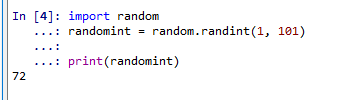
\includegraphics[width=4cm]{figures/kelompok1/1/1174021/tugas1/materi/2.PNG}
		\caption{Importing Libraries}
	\end{figure}

\subsection{Managing Files}
Managing files berfungsi untuk memungkinkan kita berinteraksi dengan sistem file, Python menyediakan kita dengan fungsi terbuka builtin. Fungsi ini dapat dipanggil untuk membuka file dan mengembalikan file objek. Itu
yang terakhir memungkinkan kita untuk melakukan berbagai operasi pada file, seperti membaca dan menulis. Setelah kita selesai berinteraksi dengan file, akhirnya kita harus ingat untuk menutupnya menggunakan metode file.close
\hfill\break
\lstinputlisting[firstline=36, lastline=45]{src/kelompok1/1174021/tugas1.py}
\hfill\break

	\begin{figure}[H]
		\centering
		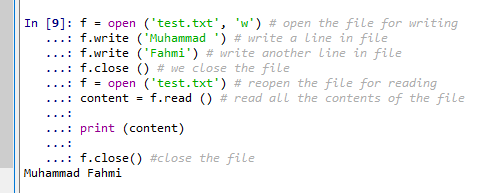
\includegraphics[width=4cm]{figures/kelompok1/1/1174021/tugas1/materi/3.PNG}
		\caption{Managing Files}
	\end{figure}

\subsection{List Comprehensions}
List comprehensions adalah alat yang ampuh untuk membuat dan memanipulasi daftar. Mereka terdiri dari ekspresi yang diikuti oleh untuk klausa dan kemudian diikuti oleh nol, atau lebih, jika klausa. Sintaksnya ialah expression for item in list. Kemudian, lakukan hal berikut:
\hfill\break
\lstinputlisting[firstline=49, lastline=56]{src/kelompok1/1174021/tugas1.py}
\hfill\break

	\begin{figure}[H]
		\centering
		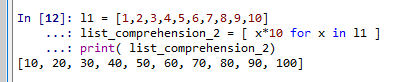
\includegraphics[width=4cm]{figures/kelompok1/1/1174021/tugas1/materi/41.PNG}
		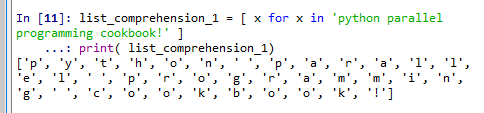
\includegraphics[width=4cm]{figures/kelompok1/1/1174021/tugas1/materi/42.PNG}
		\caption{List Comprehensions}
	\end{figure}

\subsection{Running Python Scripts}
Untuk menjalankan skrip Python, cukup panggil juru bahasa Python diikuti oleh skrip nama, dalam hal ini, mypythonscript.py. Atau, jika kita berada di direktori kerja yang berbeda, kemudian gunakan alamat lengkapnya:
\hfill\break
\lstinputlisting[firstline=58, lastline=60]{src/kelompok1/1174021/tugas1.py}
\hfill\break
Mulai sekarang, untuk setiap permintaan skrip Python, kita akan menggunakan
notasi sebelumnya; yaitu, python, diikuti oleh scriptname.py,
dengan asumsi bahwa direktori dari mana juru bahasa Python diluncurkan
adalah di mana skrip yang akan dieksekusi berada. Untuk memudahkan kita buat file python yang bernama mypythonscript.py, dengan codingan sebagai berikut, lalu buka cmd atau anaconda prompt untuk memanggil file python tersebut.
\hfill\break
\lstinputlisting[firstline=53, lastline=56]{src/kelompok1/1174021/tugas1.py}
\hfill\break

	\begin{figure}[H]
		\centering
		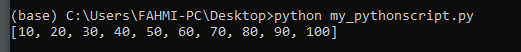
\includegraphics[width=4cm]{figures/kelompok1/1/1174021/tugas1/materi/5.PNG}
		\caption{Running Python Scripts}
	\end{figure}

\subsection{Installing Python packages using pip}
Pip adalah alat yang memungkinkan kita untuk mencari, mengunduh, dan menginstal paket Python yang ditemukan di Internet Python Package Index, yang merupakan repositori yang berisi puluhan ribu paket ditulis dengan Python. Ini juga memungkinkan kita untuk mengelola paket yang kita miliki diunduh, memungkinkan kami untuk memperbarui atau menghapusnya.
\subsubsection{Installing Pip}
Pip sudah termasuk dalam versi Python 3.4 dan 2.7.9. Untuk memeriksa apakah alat ini sudah terpasang, kita dapat menjalankan perintah berikut
\hfill\break

	\begin{figure}[H]
		\centering
		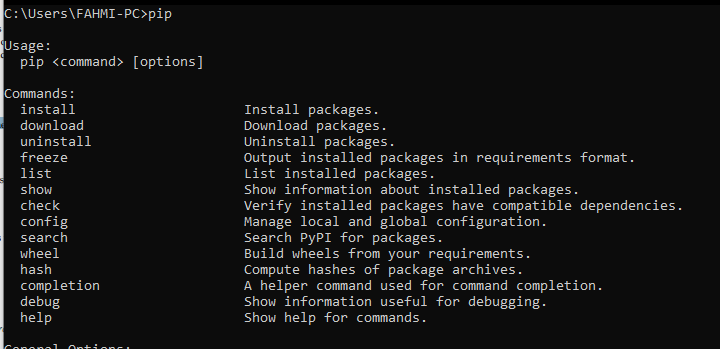
\includegraphics[width=4cm]{figures/kelompok1/1/1174021/tugas1/materi/61.PNG}
		\caption{Installing Pip}
	\end{figure}

\subsubsection{Updating Pip}
Disarankan juga untuk memeriksa bahwa versi Pip yang Anda gunakan selalu terkini. Untuk perbarui itu, kita bisa menggunakan perintah berikut:
\hfill\break

	\begin{figure}[H]
		\centering
		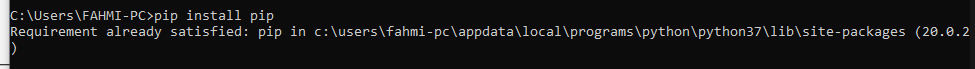
\includegraphics[width=4cm]{figures/kelompok1/1/1174021/tugas1/materi/62.PNG}
		\caption{Updating Pip}
	\end{figure}

\subsubsection{Using Pip}
Pip mendukung serangkaian perintah yang memungkinkan, antara lain, untuk mencari, mengunduh, instal, perbarui, dan hapus library. Untuk menginstal library atau modul pada python, contoh disini kita menginstall matplotlib, jalankan perintah berikut :
\hfill\break

	\begin{figure}[H]
		\centering
		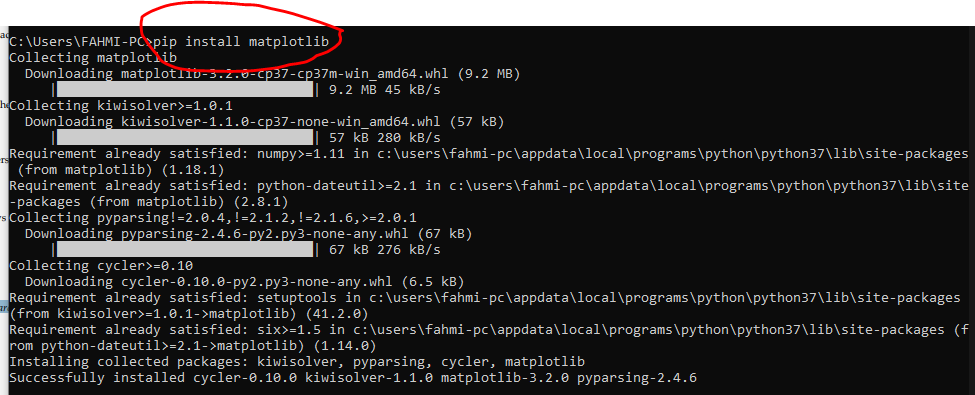
\includegraphics[width=4cm]{figures/kelompok1/1/1174021/tugas1/materi/63.PNG}
		\caption{Using Pip}
	\end{figure}
	
\subsection{Penanganan Error}
\begin{enumerate}
	\item ScreenShoot Error
	\begin{figure}[H]
		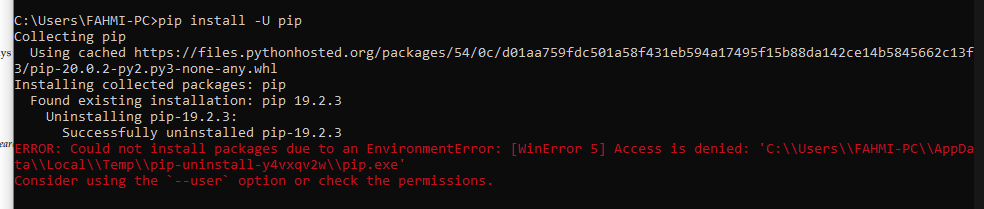
\includegraphics[width=4cm]{figures/kelompok1/1/1174021/tugas1/error/1.PNG}
		\centering
		\caption{Could not install packages}
	\end{figure}
	\item Cara Penanganan Error
	Error terdapat pada penamaan kesalahan install packages, seharusnya menghapuskan -U.
\end{enumerate}

\subsection{Bukti Tidak Plagiat}
\begin{figure}[H]
\centering
	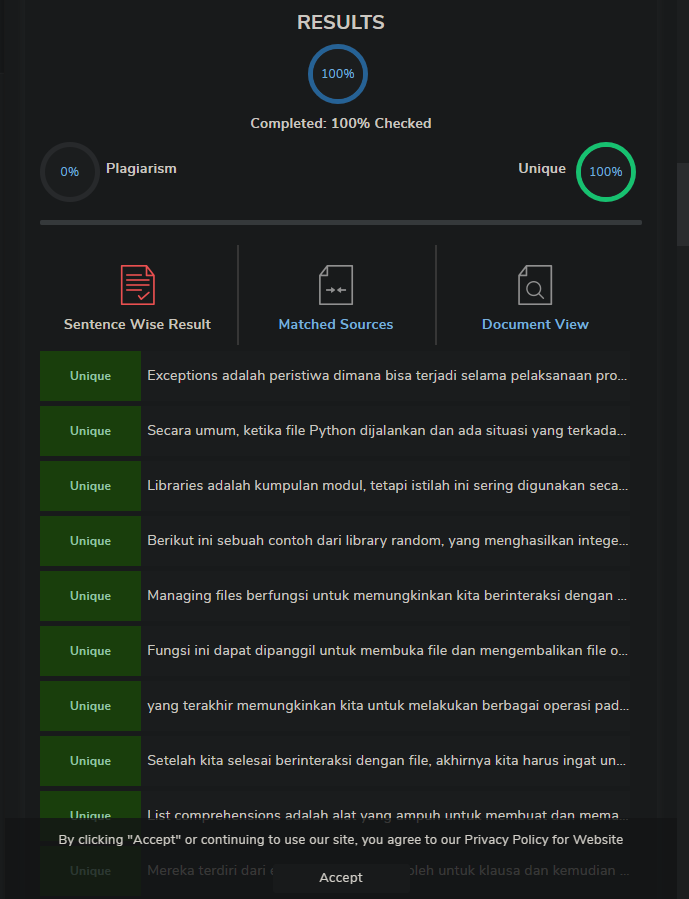
\includegraphics[width=4cm]{figures/kelompok1/1/1174021/tugas1/buktiplagiat/1.PNG}
	\caption{Bukti Tidak Melakukan Plagiat Chapter 1}
\end{figure}

\section{1174031 - Muhammad Tomy Nur Maulidy}
\subsection{Memperkenalkan pemrograman paralel Python}
	Python menyediakan banyak pustaka dan kerangka kerja yang memfasilitasi kinerja tinggi
perhitungan. Namun, melakukan pemrograman paralel dengan Python bisa sangat berbahaya
karena Global Interpreter Lock (GIL).
Bahkan, interpreter Python yang paling luas dan banyak digunakan, CPython, dikembangkan di
bahasa pemrograman C. Penerjemah CPython membutuhkan GIL untuk keamanan thread
operasi. Penggunaan GIL menyiratkan bahwa Anda akan menemukan kunci global ketika Anda mencoba
untuk mengakses objek Python yang ada di dalam utas. Dan hanya satu utas dalam satu waktu yang bisa
memperoleh kunci untuk objek Python atau API C.
Untungnya, masalahnya tidak terlalu serius, karena, di luar ranah GIL, kita bisa leluasa menggunakannya
paralelisme. Kategori ini mencakup semua topik yang akan kita bahas dalam bab-bab berikutnya,
termasuk multiprocessing, komputasi terdistribusi, dan komputasi GPU.
Jadi, Python tidak benar-benar multithreaded. Tapi apa itu utas? Apa itu proses? Dalam
bagian berikut, kami akan memperkenalkan dua konsep dasar ini dan bagaimana mereka
ditangani oleh bahasa pemrograman Python.
\subsection{Proses dan utas}
Utas dapat dibandingkan dengan proses yang ringan, dalam arti bahwa mereka menawarkan manfaat yang serupa untuk proses, tanpa, bagaimanapun, membutuhkan teknik komunikasi yang khas proses. Utilitas ini memungkinkan Anda untuk membagi aliran kontrol utama dari suatu program menjadi beberapa secara bersamaan menjalankan aliran kontrol. Sebagai gantinya, proses memiliki ruang pengalamatan sendiri dan sumber daya mereka sendiri. Kemudian komunikasi antar bagian kode berjalan Proses yang berbeda hanya dapat terjadi melalui mekanisme manajemen yang tepat, termasuk pipa, kode FIFO, kotak surat, area memori bersama, dan menyampaikan pesan. Utas, di sisi lain, memungkinkan pembuatan bagian bersamaan dari program, di mana setiap bagian dapat mengakses ruang alamat, variabel, dan konstanta yang sama.
\subsection{Praktek}
\begin{enumerate}
	\item do something
    \lstinputlisting[firstline=8, lastline=12]{src/kelompok1/do_something.py}
	\hfill\break
	\item serial test
	\hfill\break
	\lstinputlisting[firstline=8, lastline=22]{src/kelompok1/serial_test.py}
	\item multithreading test
	\hfill\break
	\lstinputlisting[firstline=8, lastline=30]{src/kelompok1/multithreading_test.py}
	\item multiprocessing test
	\hfill\break
	\lstinputlisting[firstline=8, lastline=30]{src/kelompok1/multiprocessing_testpy.py}
\end{enumerate}
\subsection{Percobaan}
\begin{enumerate}
	\item Menjalankan Serial Test
	\begin{figure}[H]
		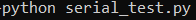
\includegraphics[width=4cm]{figures/kelompok1/1/tomy/test1.PNG}
		\centering
		\caption{Menjalankan Serial Test}
	\end{figure}
	\begin{figure}[H]
		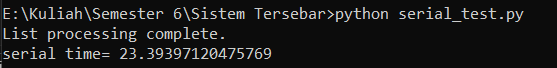
\includegraphics[width=4cm]{figures/kelompok1/1/tomy/hasil1.PNG}
		\centering
		\caption{Hasil Serial Test}
	\end{figure}
    \item Menjalankan Multithreading Test
	\begin{figure}[H]
		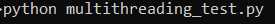
\includegraphics[width=4cm]{figures/kelompok1/1/tomy/test2.PNG}
		\centering
		\caption{Menjalankan Multithreading Test}
	\end{figure}
	\begin{figure}[H]
		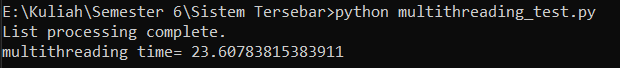
\includegraphics[width=4cm]{figures/kelompok1/1/tomy/hasil2.PNG}
		\centering
		\caption{Hasil Multithreading Test}
	\end{figure}
    \item Menjalankan Multiprocessing Test
	\begin{figure}[H]
		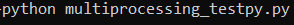
\includegraphics[width=4cm]{figures/kelompok1/1/tomy/test3.PNG}
		\centering
		\caption{Menjalankan Multiprocessing Test}
	\end{figure}
	\begin{figure}[H]
		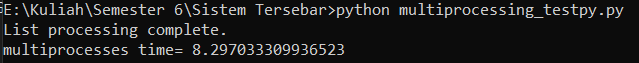
\includegraphics[width=4cm]{figures/kelompok1/1/tomy/hasil3.PNG}
		\centering
		\caption{Hasil Multiprocessing Test}
	\end{figure}
\end{enumerate}
\subsection{Bukti Tidak Plagiat}
\begin{figure}[H]
	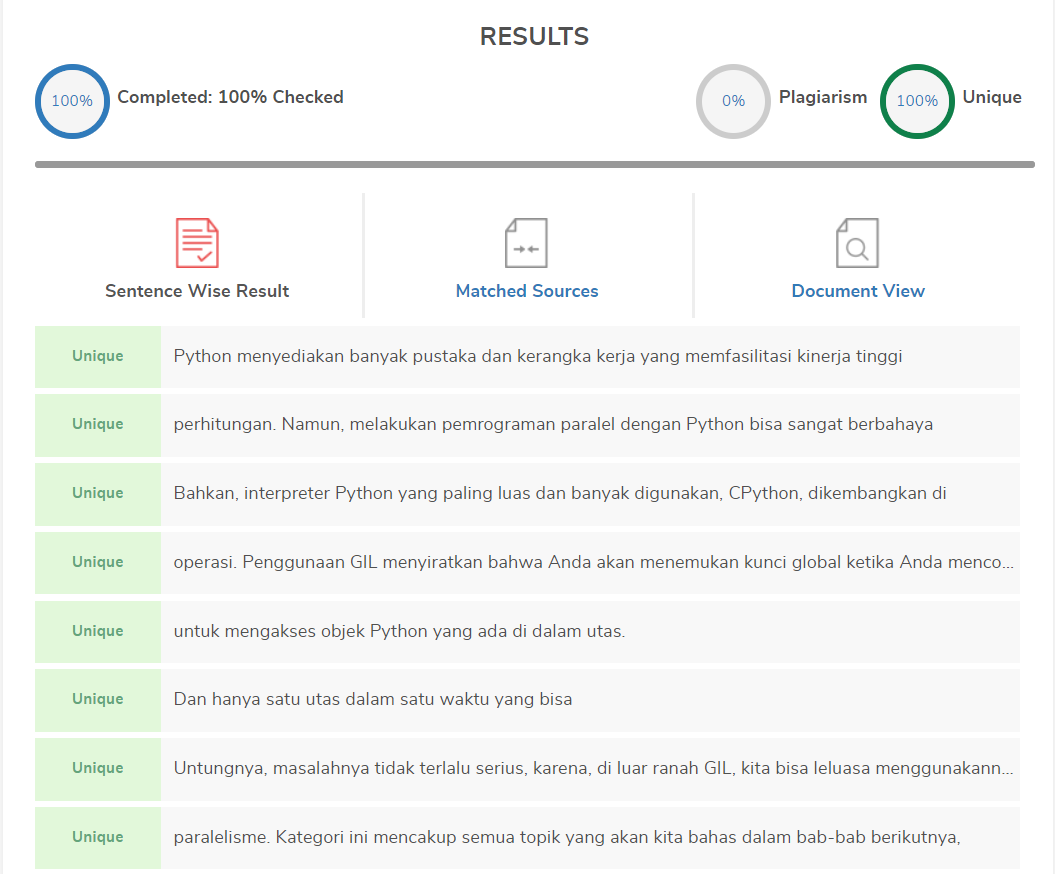
\includegraphics[width=4cm]{figures/kelompok1/1/tomy/plagiat_tomy_1.PNG}
	\centering
	\caption{Bukti Tidak Melakukan Plagiat 1}
    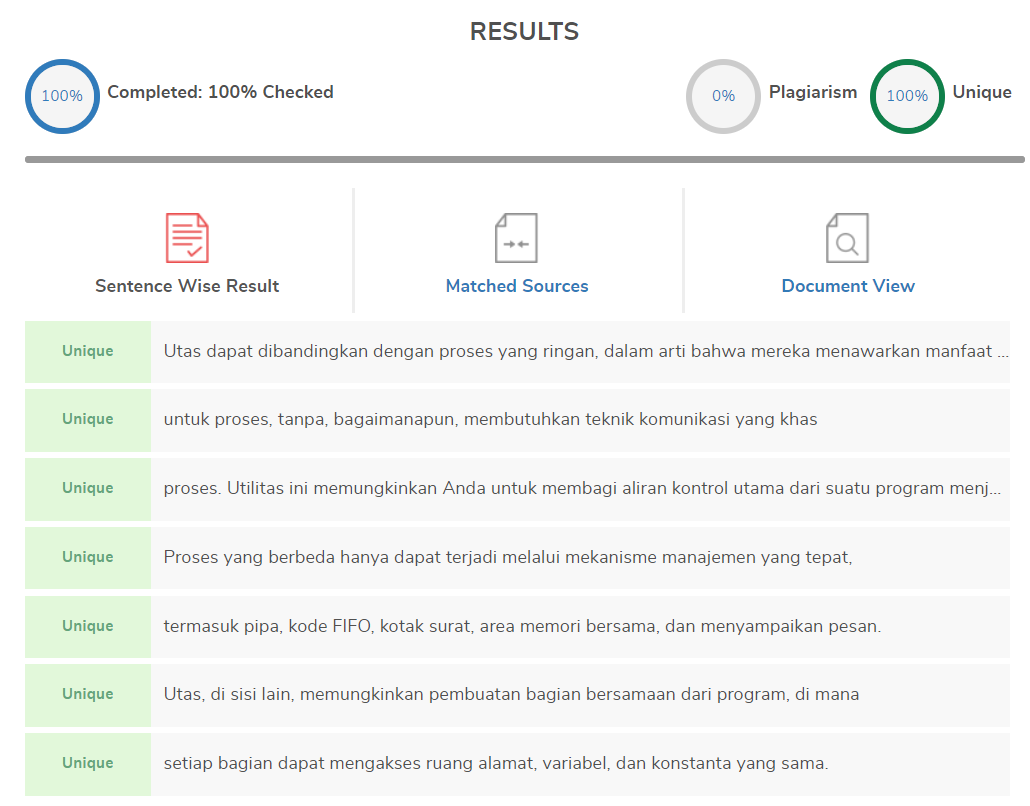
\includegraphics[width=4cm]{figures/kelompok1/1/tomy/plagiat_tomy_2.PNG}
	\centering
	\caption{Bukti Tidak Melakukan Plagiat 2}
\end{figure}

\section{Kenapa kita membutuhkan komputasi parallel?}

Pertumbuhan daya komputasi yang disediakan oleh komputer modern telah menghasilkan masalah komputasi yang semakin kompleks dalam jangka waktu yang relatif singkat. Sampai awal 2000-an, kompleksitas ditangani dengan meningkatkan jumlah transistor serta frekuensi clock dari sistem prosesor tunggal, yang mencapai puncak 3,5-4 GHz. Namun, peningkatan jumlah transistor menyebabkan peningkatan eksponensial dari daya yang dihabiskan oleh prosesor itu sendiri. Pada dasarnya, ada, oleh karena itu, keterbatasan fisik yang mencegah peningkatan lebih lanjut dalam kinerja sistem prosesor tunggal.
\noindent
Untuk alasan ini, dalam beberapa tahun terakhir, produsen mikroprosesor memusatkan perhatian mereka pada sistem multi-core. Ini didasarkan pada inti dari beberapa prosesor fisik yang berbagi memori yang sama, sehingga dengan melewatkan masalah daya yang hilang yang dijelaskan sebelumnya. Dalam beberapa tahun terakhir, sistem quad-core dan octa-core juga telah menjadi standar pada konfigurasi desktop dan laptop normal.
\noindent
Di sisi lain, perubahan signifikan dalam perangkat keras juga menghasilkan evolusi struktur perangkat lunak, yang selalu dirancang untuk dieksekusi secara berurutan pada satu prosesor. Untuk mengambil keuntungan dari sumber daya komputasi yang lebih besar yang tersedia dengan meningkatkan jumlah prosesor, perangkat lunak yang ada harus dirancang ulang dalam bentuk yang sesuai dengan struktur paralel CPU, sehingga dapat memperoleh efisiensi yang lebih besar melalui eksekusi simultan dari unit tunggal dari beberapa bagian dari program yang sama.

\section{Taksonomi Flynn}
Taksonomi Flynn adalah sistem untuk mengklasifikasikan arsitektur komputer. Ini didasarkan pada dua konsep utama:

\begin{enumerate}
	\item Instruction flow: Suatu sistem dengan n CPU memiliki n penghitung program dan, oleh karena itu, n instruksi mengalir. Ini sesuai dengan penghitung program.
	\item Data flow: Program yang menghitung fungsi pada daftar data memiliki aliran data. Program yang menghitung fungsi yang sama pada beberapa daftar data yang berbeda memiliki lebih banyak aliran data. Ini terdiri dari seperangkat operan.
\end{enumerate}

\noindent
Karena instruksi dan aliran data bersifat independen, ada empat kategori mesin paralel: Single Instruction Single Data (SISD), Single Instruction Multiple Data (SIMD), Multiple Instruction Single Data (MISD), and Multiple Instruction Multiple Data (MIMD):

\begin{figure}[H]
	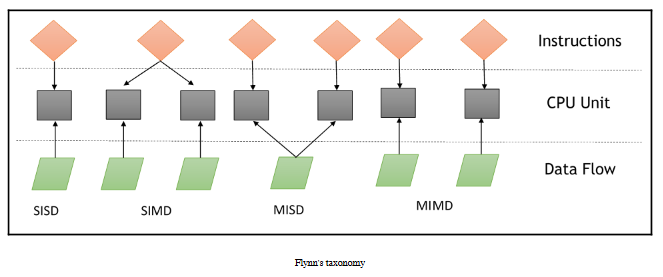
\includegraphics[width=4cm]{figures/kelompok2/chapter1/1.png}
	\centering
	\caption{Flynn.}
\end{figure}

\subsection{Single Instruction Single Data (SISD)}
Sistem komputasi SISD seperti mesin von Neumann, yang merupakan mesin uniprocessor. Seperti yang Anda lihat dalam diagram taksonomi Flynn, ia menjalankan instruksi tunggal yang beroperasi pada aliran data tunggal. Di SISD, instruksi mesin diproses secara berurutan.

\noindent
Dalam siklus clock, CPU menjalankan operasi berikut:

\begin{enumerate}
	\item Fetch: CPU mengambil data dan instruksi dari area memori, yang disebut register.
	\item Decode: CPU menerjemahkan instruksi.
	\item Execute: Instruksi dilakukan pada data. Hasil operasi disimpan dalam register lain.
\end{enumerate}

\noindent
Setelah tahap eksekusi selesai, CPU menetapkan dirinya untuk memulai siklus CPU lain:

\begin{figure}[H]
	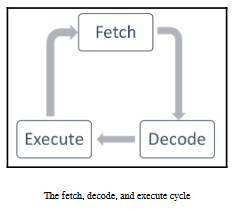
\includegraphics[width=4cm]{figures/kelompok2/chapter1/2.png}
	\centering
	\caption{SISD.}
\end{figure}

\noindent
Algoritma yang berjalan pada komputer jenis ini bersifat berurutan (atau serial) karena tidak mengandung paralelisme. Contoh komputer SISD adalah sistem perangkat keras dengan satu CPU.

\noindent
Elemen utama dari arsitektur ini (yaitu, arsitektur von Neumann) adalah sebagai berikut:

\begin{enumerate}
	\item Central memori unit: Ini digunakan untuk menyimpan instruksi dan data program.
	\item CPU: Ini digunakan untuk mendapatkan instruksi dan / atau data dari unit memori, yang menerjemahkan instruksi dan secara berurutan mengimplementasikannya.
	\item The I/O system: Ini mengacu pada data input dan output dari program.
\end{enumerate}

\noindent
Komputer prosesor tunggal konvensional diklasifikasikan sebagai sistem SISD:

\begin{figure}[H]
	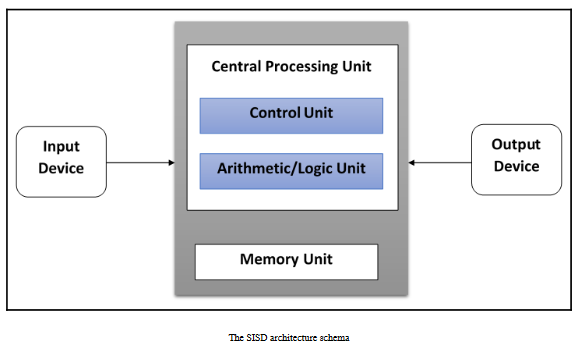
\includegraphics[width=4cm]{figures/kelompok2/chapter1/3.png}
	\centering
	\caption{Algoritma SISD.}
\end{figure}

\noindent
Diagram berikut secara khusus menunjukkan area mana dari CPU yang digunakan pada tahap pengambilan, dekode, dan eksekusi:

\begin{figure}[H]
	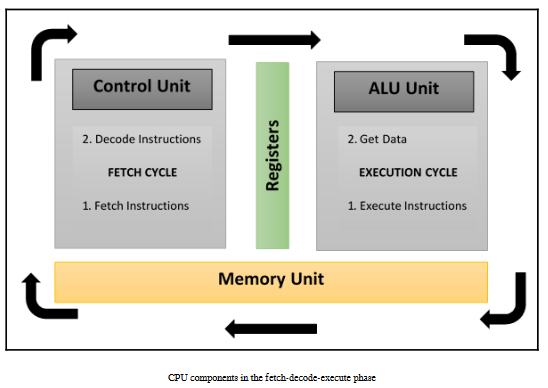
\includegraphics[width=4cm]{figures/kelompok2/chapter1/4.png}
	\centering
	\caption{Area Fetch CPU.}
\end{figure}

\subsection{MISD}
\textit{Multiple Instruction Single Data} \textbf{(MISD)}. Dalam model ini, prosesor, masing-masing dengan unit kontrol mereka sendiri, berbagi unit memori tunggal. Dalam setiap siklus clock, data yang diterima dari memori diproses oleh semua prosesor secara bersamaan, masing-masing sesuai dengan instruksi yang diterima dari unit kontrol. Dalam hal ini, paralelisme (paralelisme tingkat instruksi) diperoleh dengan melakukan beberapa operasi pada bagian data yang sama. Jenis masalah yang dapat dipecahkan secara efisien dalam arsitektur ini agak istimewa, seperti enkripsi data. Untuk alasan ini, komputer MISD belum menemukan ruang di sektor komersial. Komputer MISD lebih dari satu latihan intelektual daripada konfigurasi praktis

\subsection{SIMD}
\textit{Single Instruction Multiple Data} \textbf{(SIMD)}. Sebuah SIMD komputer terdiri dari n prosesor yang identik, masing-masing dengan memori lokal mereka sendiri, di mana dimungkinkan untuk menyimpan data. Semua prosesor bekerja di bawah kendali aliran instruksi tunggal. Selain itu, ada n data stream, satu untuk setiap prosesor. Prosesor bekerja secara simultan pada setiap langkah dan menjalankan instruksi yang sama, tetapi pada elemen data yang berbeda. Ini adalah contoh dari data tingkat paralelisme.
SIMD arsitektur jauh lebih fleksibel daripada arsitektur MISD. Banyak masalah yang mencakup berbagai macam aplikasi dapat diselesaikan dengan algoritma paralel pada komputer SIMD. Fitur lain yang menarik adalah bahwa algoritma untuk komputer ini relatif mudah untuk merancang, menganalisis, dan menerapkan. pembatasan adalah bahwa hanya masalah yang dapat dibagi menjadi beberapa submasalah (yang semuanya identik, yang masing-masing kemudian akan diselesaikan secara simultan melalui set instruksi yang sama) dapat diatasi dengan komputer SIMD.
\subsection{MIMD}
\textit{Multiple Instruction Multiple Data} \textbf{MIMD}. kelas ini merupakan kelas umum dan paling kuat, menurut klasifikasi Flynn. Ini mengandung prosesor, instruksi stream, dan data stream. Setiap prosesor memiliki satuan sendiri kontrol dan memori lokal, yang membuat MIMD arsitektur lebih komputasi kuat dari arsitektur SIMD.
Setiap prosesor beroperasi di bawah kendali aliran instruksi yang dikeluarkan oleh unit kontrol sendiri. Oleh karena itu, prosesor berpotensi dapat menjalankan program yang berbeda dengan data yang berbeda, yang memungkinkan mereka untuk memecahkan submasalah yang berbeda dan dapat menjadi bagian dari masalah yang lebih besar tunggal. Dalam MIMD, arsitektur dicapai dengan bantuan tingkat paralelisme dengan benang dan / atau proses. Ini juga berarti bahwa prosesor biasanya beroperasi asynchronous.

Saat ini, arsitektur ini diterapkan untuk banyak PC, superkomputer, dan jaringan komputer. Namun, ada counter yang perlu Anda pertimbangkan: algoritma asynchronous sulit untuk merancang, menganalisis, dan menerapkan:

\begin{figure}[H]
	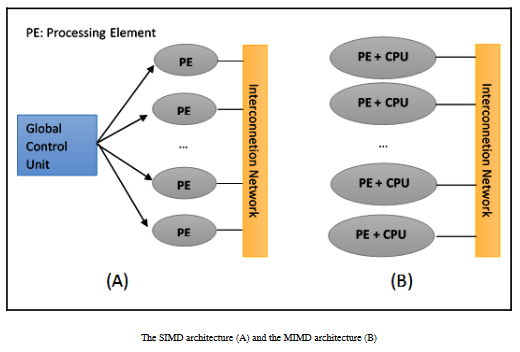
\includegraphics[width=4cm]{figures/kelompok2/chapter1/5.png}
	\centering
	\caption{MIMD.}
\end{figure}

\section{Organisasi Memori}
Aspek lain yang perlu kita pertimbangkan dalam rangka untuk mengevaluasi arsitektur paralel organisasi memori, atau lebih tepatnya, cara di mana data yang diakses. Tidak peduli seberapa cepat unit pengolahan, jika memori tidak dapat mempertahankan dan memberikan petunjuk dan data pada kecepatan yang cukup, maka tidak akan ada peningkatan kinerja. Masalah utama yang kita butuhkan untuk mengatasi untuk membuat waktu respon dari memori yang kompatibel dengan kecepatan prosesor adalah memori waktu siklus, yang didefinisikan sebagai waktu yang telah berlalu antara dua operasi berturut-turut. Waktu siklus prosesor biasanya lebih singkat daripada waktu siklus memori.

Ketika prosesor memulai transfer ke atau dari memori, sumber daya prosesor akan tetap diduduki untuk seluruh durasi siklus memori; Selanjutnya, selama periode ini, tidak ada perangkat lain (misalnya, I / O controller, prosesor, atau bahkan prosesor yang membuat permintaan) akan dapat menggunakan memori karena transfer berlangsung:
Masalahnya terjadi ketika prosesor memodifikasi data yang disimpan dalam sistem memori itu secara bersamaan digunakan oleh prosesor lain. Nilai baru akan lulus dari cache prosesor yang telah diubah ke memori bersama. Namun kemudian, itu juga harus diteruskan ke semua prosesor lainnya, sehingga mereka tidak bekerja dengan nilai usang. Masalahnya adalah dikenal sebagai masalah koherensi cache — kasus khusus dari masalah memori konsistensi, yang memerlukan implementasi perangkat keras yang dapat menangani masalah konkurensi dan sinkronisasi, mirip dengan pemrograman thread.

Fitur utama dari sistem memori bersama adalah sebagai berikut: Memori sama untuk semua prosesor. Misalnya, semua prosesor terkait dengan struktur data yang sama akan bekerja dengan memori logis yang sama alamat, sehingga mengakses lokasi memori yang sama. Sinkronisasi diperoleh dengan membaca tugas berbagai prosesor dan memungkinkan memori bersama. Bahkan, prosesor hanya dapat mengakses satu memori pada suatu waktu. Lokasi memori bersama tidak boleh diubah dari tugas sementara tugas lain mengaksesnya. Berbagi data antar tugas dengan cepat. Waktu yang dibutuhkan untuk berkomunikasi adalah waktu yang diperlukan salah satu dari mereka untuk membaca satu lokasi (tergantung pada kecepatan akses memori).

Akses memori dalam sistem memori bersama adalah sebagai berikut :
\begin{enumerate}
\item Akses memori dalam sistem memori bersama adalah sebagai berikut: 
\item Uniform Memory Access (UMA): Karakteristik mendasar dari sistem ini adalah waktu akses ke memori yang konstan untuk setiap prosesor dan untuk apa saja area memori. Untuk alasan ini, sistem ini juga disebut Simetris Multiprosesor (SMP). Mereka relatif sederhana untuk diterapkan, tetapi tidak terlalu terukur. Coder bertanggung jawab atas pengelolaan sinkronisasi oleh memasukkan kontrol yang sesuai, semaphores, mengunci, dan lainnya di program itu mengelola sumber daya
\item Non-Uniform Memory Access (NUMA): Arsitektur ini membagi memori ke area akses berkecepatan tinggi yang ditugaskan untuk setiap prosesor, dan juga, a area umum untuk pertukaran data, dengan akses yang lebih lambat. Sistem ini juga disebut sistem Distributed Shared Memory (DSM). Mereka sangat scalable, tetapi kompleks untuk dikembangkan. 
\item Tidak Ada Akses Memori Jarak Jauh (NoRMA): Memori didistribusikan secara fisik di antara prosesor (memori lokal). Semua kenangan lokal bersifat pribadi dan bisa hanya mengakses prosesor lokal. Komunikasi antara prosesor adalah melalui protokol komunikasi yang digunakan untuk bertukar pesan, yaitu dikenal sebagai protokol penyampaian pesan.
\item Cache-Only Memory Arsitektur (Koma): Sistem ini dilengkapi dengan kenangan hanya cache. Sementara menganalisis arsitektur NUMA, itu menyadari bahwa arsitektur ini terus salinan lokal dari data dalam cache dan data ini disimpan sebagai duplikat dalam memori utama. Arsitektur ini menghilangkan duplikat dan membuat hanya kenangan cache; memori didistribusikan secara fisik antara prosesor (memori lokal). Semua kenangan lokal pribadi dan hanya dapat mengakses prosesor lokal. Komunikasi antara prosesor juga melalui protokol pesan-lewat.
\end{enumerate}
\begin{figure}[H]
	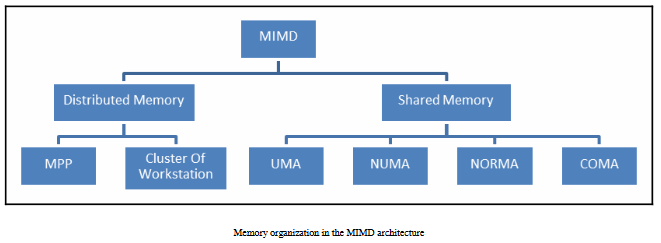
\includegraphics[width=4cm]{figures/kelompok2/chapter1/6.png}
	\centering
	\caption{Memory Organization.}
\end{figure}

\subsection{Shared Memory}

\begin{figure}[H]
	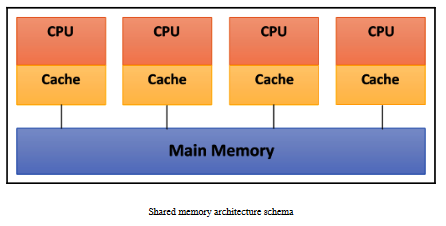
\includegraphics[width=4cm]{figures/kelompok2/chapter1/7.png}
	\centering
	\caption{Shared Memory.}
\end{figure}

\subsection{Distributed Memory}
 Dalam sistem dengan memori terdistribusi, memori dikaitkan dengan masing-masing prosesor dan sebuah prosesor hanya mampu mengatasi memori sendiri. Beberapa penulis menyebut jenis sistem sebagai multicomputer suatu, mencerminkan fakta bahwa unsur-unsur dari sistem ini adalah, sendiri, sistem yang kecil dan lengkap dari prosesor dan memori, seperti yang Anda lihat pada diagram berikut:
\begin{figure}[H]
	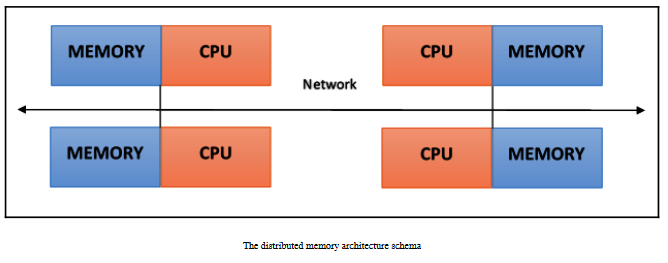
\includegraphics[width=4cm]{figures/kelompok2/chapter1/8.png}
	\centering
	\caption{Distributed Memory.}
\end{figure}
\noindent
organisasi semacam ini memiliki beberapa keunggulan:

\begin{enumerate}
	\item Tidak ada konflik di tingkat bus komunikasi atau switch. Setiap prosesor dapat menggunakan bandwidth penuh memori lokal mereka sendiri tanpa campur tangan dari prosesor lainnya.
	\item Kurangnya sarana bus umum yang tidak ada batas intrinsik untuk jumlah prosesor. Ukuran sistem ini hanya dibatasi oleh jaringan yang digunakan untuk menghubungkan prosesor.
	\item Tidak ada masalah dengan koherensi cache. Setiap prosesor bertanggung jawab untuk data sendiri dan tidak harus khawatir tentang upgrade salinan apapun.

Kerugian utama adalah bahwa komunikasi antara prosesor lebih sulit untuk menerapkan. Jika prosesor membutuhkan data dalam memori prosesor lain, maka dua prosesor tidak harus selalu bertukar pesan melalui protokol pesan-lewat. Ini memperkenalkan dua sumber perlambatan: untuk membangun dan mengirim pesan dari satu prosesor ke yang lain membutuhkan waktu, dan juga, setiap prosesor harus dihentikan untuk mengelola pesan yang diterima dari prosesor lainnya. Sebuah program yang dirancang untuk bekerja pada mesin memori terdistribusi harus diselenggarakan sebagai satu set tugas independen yang berkomunikasi melaluipesan:
\end{enumerate}

\begin{figure}[H]
	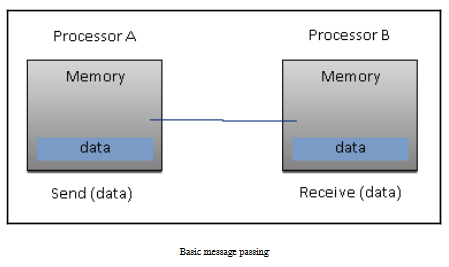
\includegraphics[width=4cm]{figures/kelompok2/chapter1/9.png}
	\centering
	\caption{Distributed Memory 2.}
\end{figure}

\noindent
Fitur utama dari sistem memori terdistribusi adalah sebagai berikut:

\begin{enumerate}
	\item Memori secara fisik didistribusikan antara prosesor; setiap memori lokal secara langsung dapat diakses hanya dengan prosesor.
	\item Sinkronisasi dicapai dengan memindahkan data (bahkan jika itu hanya pesan itu sendiri) antara prosesor (komunikasi).
	\item Subdivisi data dalam kenangan lokal mempengaruhi kinerja mesin-adalah penting untuk membuat subdivisi akurat, sehingga dapat meminimalkan komunikasi antara CPU. Selain itu, prosesor yang koordinat operasi ini dekomposisi dan komposisi harus berkomunikasi secara efektif dengan prosesor yang beroperasi pada bagian-bagian individu dari struktur data.
         \item Protokol message-passing digunakan sehingga CPU dapat berkomunikasi satu sama lain melalui pertukaran paket data. Pesan adalah unit diskrit informasi, dalam arti bahwa mereka memiliki identitas yang jelas, sehingga selalu mungkin untuk membedakan mereka dari satu sama lain.


\subsection{MPP}
mesin MPP terdiri dari ratusan prosesor (yang dapat sebagai besar sebagai ratusan ribu prosesor di beberapa mesin) yang terhubung oleh jaringan komunikasi. Komputer tercepat di dunia didasarkan pada arsitektur ini; beberapa contoh dari sistem arsitektur ini Earth Simulator, Blue Gene, ASCI White, ASCI Merah, dan ASCI Purple dan Red Storm-storm.

\subsection{Clusters of Workstations}
\item Sistem pengolahan didasarkan pada komputer klasik yang dihubungkan oleh jaringan komunikasi. cluster komputasi jatuh ke dalam klasifikasi ini.
\item Dalam arsitektur cluster, kita mendefinisikan node sebagai unit komputasi tunggal yang mengambil bagian dalam cluster. Untuk pengguna, cluster sepenuhnya transparan-semua perangkat keras dan perangkat lunak kompleksitas bertopeng dan data dan aplikasi yang dibuat dapat diakses seolah-olah mereka semua dari node tunggal.
\noindent Di sini, kami telah mengidentifikasi tiga jenis kelompok:
\item Gagal-lebih klaster: Dalam hal ini, kegiatan node terus dipantau, dan ketika salah satu berhenti bekerja, komputer lain mengambil alih jawab kegiatan tersebut. Tujuannya adalah untuk memastikan layanan terus menerus karena redundansi dari arsitektur yang baik.
\item Load balancing klaster: Dalam sistem ini, permintaan pekerjaan dikirim ke node yang memiliki kurang aktivitas. waktu Memastikan bahwa kurang ini diambil untuk memproses pekerjaan.
\item Kinerja tinggi komputasi klaster: Dalam hal ini, setiap node dikonfigurasi untuk memberikan kinerja yang sangat tinggi. Proses ini juga dibagi menjadi beberapa pekerjaan di beberapa node. Pekerjaan yang diparalelkan dan akan didistribusikan ke mesin yang berbeda.




\subsection{Heterogeneous Architectures}
Pengenalan akselerator GPU di dunia homogen superkomputer telah mengubah sifat bagaimana superkomputer keduanya digunakan dan diprogram sekarang. Meskipun kinerja tinggi yang ditawarkan oleh GPU, mereka tidak dapat dianggap sebagai unit pengolahan otonom karena mereka harus selalu disertai dengan kombinasi CPU. Paradigma pemrograman, karena itu, adalah sangat sederhana: CPU mengambil kendali dan hitungan secara serial, menetapkan tugas untuk akselerator grafis yang, komputasi, sangat mahal dan memiliki tingkat tinggi paralelisme yang baik.
\item Komunikasi antara CPU dan GPU dapat berlangsung, tidak hanya melalui penggunaan bus berkecepatan tinggi tetapi juga melalui berbagi satu daerah memori untuk memori fisik atau virtual. Bahkan, dalam kasus di mana kedua perangkat tidak dilengkapi dengan area memori mereka sendiri, adalah mungkin untuk mengacu pada area memori umum menggunakan perpustakaan software yang disediakan oleh berbagai model pemrograman, seperti CUDA dan OpenCL.
\item arsitektur ini disebut arsitektur heterogen, dimana aplikasi dapat membuat struktur data dalam ruang alamat tunggal dan mengirim pekerjaan ke perangkat keras, yang sesuai untuk resolusi tugas. Beberapa tugas pengolahan dapat beroperasi dengan aman di daerah yang sama untuk menghindari masalah konsistensi data, berkat operasi atom.
\item Jadi, terlepas dari kenyataan bahwa CPU dan GPU tampaknya tidak bekerja secara efisien bersama, dengan penggunaan arsitektur baru ini, kami dapat mengoptimalkan interaksi mereka dengan, dan kinerja, aplikasi paralel:



\begin{figure}[H]
	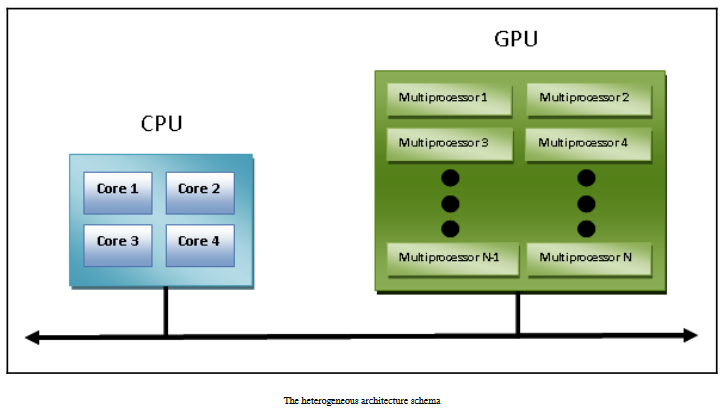
\includegraphics[width=4cm]{figures/kelompok2/chapter1/10.png}
	\centering
	\caption{Architectures.}
\end{figure}
\section{1174009 - Dwi Yulianingsih}
\subsection{Parallel Programming Models}
\hfill\break
Model pemrograman paralel ada sebagai abstraksi arsitektur perangkat keras dan memori. Faktanya, model ini tidak spesifik dan tidak merujuk pada jenis mesin atau arsitektur memori tertentu. Mereka dapat diimplementasikan (setidaknya secara teoritis) pada semua jenis mesin. Dibandingkan dengan subdivisi sebelumnya, model pemrograman ini dibuat pada tingkat yang lebih tinggi dan mewakili cara di mana perangkat lunak harus diimplementasikan untuk melakukan perhitungan paralel. Setiap model memiliki caranya sendiri untuk berbagi informasi dengan prosesor lain untuk mengakses memori dan membagi pekerjaan. Secara absolut, tidak ada satu model yang lebih baik dari yang lain. Oleh karena itu, solusi terbaik untuk diterapkan akan sangat tergantung pada masalah yang harus ditangani dan diselesaikan oleh seorang programmer. 
Model yang paling banyak digunakan untuk pemrograman paralel adalah sebagai berikut: 
\begin{itemize}
	\item Model memori bersama 
	\item Model multithread 
	\item Model distribusi memori / pesan terdistribusi
	\item Model paralel data 
\end{itemize}
Dalam resep ini, kami akan memberi Anda gambaran umum tentang model-model ini.
 \begin{figure}[H]
        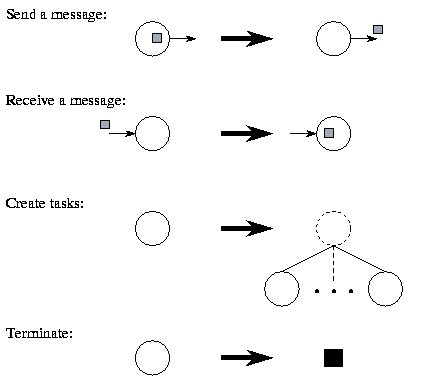
\includegraphics[width=4cm]{figures/kelompok3/1/dwi1.PNG}
        \centering
        \caption{PPM}
\end{figure}
\hfill\break
\subsection{Shared Memory Models}
\hfill\break
Dalam model ini, tugas berbagi area memori tunggal di mana kita dapat membaca dan menulis secara tidak sinkron. Ada mekanisme yang memungkinkan pembuat kode untuk mengontrol akses ke memori bersama; misalnya, mengunci atau semafor. Model ini menawarkan keuntungan bahwa pembuat kode tidak perlu mengklarifikasi komunikasi antar tugas. Kerugian penting, dalam hal kinerja, adalah menjadi lebih sulit untuk memahami dan mengelola lokalitas data. Ini mengacu pada menjaga data tetap lokal untuk prosesor yang bekerja pada menghemat akses memori, penyegaran cache, dan lalu lintas bus yang terjadi ketika beberapa prosesor menggunakan data yang sama.
 \begin{figure}[H]
        \includegraphics[width=4cm]{figures/kelompok3/1/dwi11.PNG}
        \centering
        \caption{SMM}
\end{figure}
\hfill\break
\subsection{Multithread Models}
\hfill\break
Dalam model ini, suatu proses dapat memiliki beberapa alur eksekusi. Misalnya, bagian berurutan dibuat dan, kemudian, serangkaian tugas dibuat yang dapat dieksekusi secara paralel. Biasanya, model jenis ini digunakan pada arsitektur memori bersama. Jadi, akan sangat penting bagi kita untuk mengelola sinkronisasi antara utas, karena mereka beroperasi pada memori bersama, dan programmer harus mencegah beberapa utas dari memperbarui lokasi yang sama pada saat yang sama. CPU generasi sekarang multithreaded dalam perangkat lunak dan perangkat keras. Utas POSIX (kependekan dari Portable Operating System Interface) adalah contoh klasik dari implementasi multithreading pada perangkat lunak. Teknologi Hyper-Threading Intel mengimplementasikan multithreading pada perangkat keras dengan beralih di antara dua utas saat seseorang terhenti atau menunggu di I / O. Paralelisme dapat dicapai dari model ini, bahkan jika penyelarasan data nonlinier.
 \begin{figure}[H]
        \includegraphics[width=4cm]{figures/kelompok3/1/dwi3.PNG}
        \centering
        \caption{MM}
\end{figure}
\hfill\break
\subsection{Message Passing Models}
\hfill\break
Model pesan lewat biasanya diterapkan dalam kasus di mana setiap prosesor memiliki memori sendiri (sistem memori terdistribusi). Lebih banyak tugas dapat berada di mesin fisik yang sama atau pada jumlah mesin yang sewenang-wenang. Coder bertanggung jawab untuk menentukan paralelisme dan pertukaran data yang terjadi melalui pesan, dan perlu untuk meminta dan memanggil pustaka fungsi dalam kode. Beberapa contoh sudah ada sejak tahun 1980-an, tetapi hanya pada pertengahan 1990-an adalah model standar yang dibuat, mengarah ke standar de facto yang disebut Message Passing Interface (MPI).
 \begin{figure}[H]
        \includegraphics[width=4cm]{figures/kelompok3/1/dwi4.PNG}
        \centering
        \caption{MPM}
\end{figure}

\section{1174003 - Dwi Septiani Tsaniyah}
\subsection{Data Parallel Model}
\hfill\break
Didalam model ini lebih banyak tugas yang beroperasi pada structure data yang sama , tetapi masuk ke dalam masing-masing tugasnya. Model ini beroperasi pada bagian data yang berbeda , tetapi dalam arsitektur memori bersama , semua tugas memiliki akses data melalui memori , dimana struktur data dibagi dan berada di memori lokal di setiap tugas. Untuk menerapkan model ini, seorang pembuat kode harus mengembangkan program yang menentukan distribusi dan penyelarasan data; misalnya, GPU generasi saat ini sangat operasional 
Dalam resep ini, kami akan memberi Anda gambaran umum tentang model-model ini.
 \begin{figure}[H]
        \includegraphics[width=4cm]{figures/kelompok3/1/septi.jpg}
        \centering
        \caption{DPM}
\end{figure}
\subsection{Merancang Program Data Parallel}
\hfill\break
Desain algoritma yang mengeksploitasi paralelisme didasarkan pada serangkaian operasi, yang harus dilakukan agar program dapat melakukan pekerjaan dengan benar tanpa menghasilkan sebagian atau hasil yang salah. Operasi makro yang harus dilakukan untuk yang benar paralelisasi suatu algoritma adalah sebagai berikut:
\begin{itemize}
	\item Dekomposisi 
	\item Penugasan
	\item Pengelompokan
	\item Pemetaan
\end{itemize}

\section{1174008 - Arjun Yuda Firwanda}
\subsection{Komputasi Paralel}
\hfill\break
Pertumbuhan daya komputasi yang disediakan oleh komputer modern telah mengakibatkan kami menghadapi masalah komputasi yang semakin kompleks dalam jangka waktu yang relatif singkat. Sampai awal 2000-an, kompleksitas ditangani dengan meningkatkan jumlah transistor serta frekuensi clock dari sistem prosesor tunggal, yang mencapai puncak 3,5-4 GHz. Namun, peningkatan jumlah transistor menyebabkan peningkatan eksponensial dari daya yang dihabiskan oleh prosesor itu sendiri.

\hfill\break
\subsection{Taksonomi Flynn }
\hfill\break
Taksonomi Flynn adalah sistem untuk mengklasifikasikan arsitektur komputer. Ini didasarkan pada dua konsep utama:
\begin{itemize}
	\item Alur instruksi: Suatu sistem dengan n CPU memiliki n penghitung program dan sesuai dengan penghitung program.
	\item Aliran data: Program yang menghitung fungsi pada daftar data memiliki aliran data.
\end{itemize}
\hfill\break
    \begin{figure}[H]
        \includegraphics[width=4cm]{figures/kelompok3/1/arjun1.png}
        \centering
        \caption{tf}
    \end{figure}
Ada empat kategori mesin paralel: Instruksi Tunggal, Data Tunggal (SISD), Data Instruksi Berganda (SIMD), Instruksi Berganda Data Tunggal (MISD), dan Data Instruksi Berganda Banyak (MIMD).


\subsection{Single Instruction Single Data}
\hfill\break
Single Instruction Single Data (SISD) Sistem komputasi SISD seperti mesin von Neumann, yang merupakan mesin uniprocessor. 
Dalam siklus clock, CPU menjalankan operasi berikut:
\begin{itemize}
	\item Fetch: CPU mengambil data dan instruksi dari area memori, yang disebut register.
	\item Decode: CPU menerjemahkan instruksi.
	\item Execute: Instruksi dilakukan pada data. Hasil operasi disimpan dalam register lain.
\end{itemize}
\hfill\break
    \begin{figure}[H]
        \includegraphics[width=4cm]{figures/kelompok3/1/arjun2.png}
        \centering
        \caption{sisd}
    \end{figure}
\hfill\break
Elemen utama dari arsitektur ini (yaitu, arsitektur von Neumann) adalah sebagai berikut:
\begin{itemize}
	\item Unit memori pusat: Ini digunakan untuk menyimpan instruksi dan data program.
	\item CPU: Ini digunakan untuk mendapatkan instruksi dan / atau data dari unit memori, yang menerjemahkan instruksi dan secara berurutan mengimplementasikannya.
	\item Sistem I atau  O: Ini mengacu pada data input dan output dari program..
\end{itemize}

\section{1174096 - Nico Ekklesia Sembiring}
\subsection{Percepatan/speedup}
Percepatan adalah ukuran yang menampilkan manfaat dari penyelesaian masalah secara paralel. Percepatan didefinisikan sebagai rasio waktu yang dibutuhkan untuk menyelesaikan masalah pada elemen pemrosesan tunggal (Ts) dengan waktu yang dibutuhkan untuk memecahkan masalah yang sama pada p identik elemen pemrosesan (Tp).
\begin{figure}[H]
    \includegraphics[width=4cm]{figures/kelompok3/1/speedup.png}
    \centering
    \caption{Rumus Percepatan}
\end{figure}
jika S = p, maka itu berarti bahwa kecepatan eksekusi meningkat dengan jumlah prosesor. Tentu saja, ini adalah kasus yang ideal. Sementara speedup mutlak ketika Ts adalah waktu eksekusi dari algoritma sekuensial terbaik, speedup relatif ketika Ts adalah waktu eksekusi dari algoritma paralel untuk satu prosesor. 
\hfill\break
Mari kita rekap kondisi ini
\begin{enumerate}
	\item S = p adalah percepatan linier atau ideal. 
	\item S <p adalah percepatan nyata. 
	\item S> p adalah percepatan superlinear.
\end{enumerate}

\subsection{Efisiensi}
Sistem parallel dengan elemen pemrosesan p dapat memberi kita kecepatan yang sama dengan p. Namun, ini sangat jarang dicapai. Biasanya, beberapa waktu terbuang baik dalam pemalasan atau berkomunikasi. 
\hfill\break
Efisiensi adalah ukuran dari seberapa banyak waktu eksekusi yang dilakukan oleh elemen pemrosesan untuk melakukan pekerjaan yang bermanfaat, diberikan sebagai sebagian kecil dari waktu yang dihabiskan.

\begin{figure}[H]
    \includegraphics[width=4cm]{figures/kelompok3/1/efisiensi.png}
    \centering
    \caption{Rumus Efisiensi}
\end{figure}
Algoritma dengan speedup linier memiliki nilai E = 1. Dalam kasus lain, terdapat nilai E kurang dari 1. 
\hfill\break
Tiga kasus diidentifikasi sebagai berikut:
\begin{enumerate}
	\item Ketika E = 1, itu adalah kasus linier.  
	\item Ketika E <1, itu adalah kasus nyata.  
	\item Ketika E << 1, itu adalah masalah yang dapat diparalelkan dengan efisiensi rendah.
\end{enumerate}
\subsection{Penskalaan(Scaling)}
Penskalaan didefinisikan sebagai kemampuan untuk menjadi efisien pada mesin paralel. Ini mengidentifikasi kekuatan komputasi (kecepatan eksekusi) secara proporsional dengan jumlah prosesor. Dengan meningkatkan ukuran masalah dan, pada saat yang sama, jumlah prosesor, tidak akan ada kerugian dalam hal kinerja. Sistem yang dapat diskalakan, tergantung pada peningkatan faktor yang berbeda, dapat mempertahankan efisiensi yang sama atau meningkatkannya.

\subsection{Hukum Amdahl}
Hukum Amdahl adalah hukum yang banyak digunakan yang digunakan untuk merancang prosesor dan algoritma paralel. Ini menyatakan bahwa speedup maksimum yang dapat dicapai dibatasi oleh komponen serial program:
\begin{figure}[H]
    \includegraphics[width=4cm]{figures/kelompok3/1/amdahl.png}
    \centering
    \caption{Rumus Hukum Amdahl}
\end{figure}
1 - P menunjukkan komponen serial (tidak diparalelkan) dari suatu program.
\hfill\break
Ini berarti bahwa, misalnya, jika suatu program di mana 90% dari kode dapat dibuat paralel, tetapi 10% harus tetap serial, maka speedup maksimum yang dapat dicapai adalah 9, bahkan untuk jumlah prosesor yang tak terbatas.

\subsection{Hukum Gustafson}
Rumus hukum Gustafson adalah sebagai berikut : 
\begin{figure}[H]
    \includegraphics[width=4cm]{figures/kelompok3/1/gustafson.png}
    \centering
    \caption{Rumus Hukum Gustafson}
\end{figure}
Pada persamaan berikut ini berlaku:
\begin{enumerate}
	\item P adalah jumlah prosesor.  
	\item S adalah faktor percepatan.  
	\item alpha adalah fraksi yang tidak dapat diparalelkan dari setiap proses paralel.
\end{enumerate}
Hukum Gustafson berbeda dengan hukum Amdahl, yang mengasumsikan bahwa keseluruhan beban kerja suatu program tidak berubah sehubungan dengan jumlah prosesor.
\hfill\break
Faktanya, hukum Gustafson menyatakan bahwa programmer pertama-tama mengatur waktu yang diizinkan untuk menyelesaikan masalah secara paralel dan kemudian berdasarkan pada hal itu (yaitu waktu) untuk mengukur masalah. Oleh karena itu, semakin cepat sistem paralelnya, semakin besar masalah yang dapat diselesaikan selama periode waktu yang sama.
\hfill\break
Efek dari hukum Gustafson adalah untuk mengarahkan tujuan penelitian komputer ke arah pemilihan atau perumusan kembali masalah sedemikian rupa sehingga solusi dari masalah yang lebih besar masih mungkin dalam jumlah waktu yang sama. Selanjutnya, undang-undang ini mendefinisikan kembali konsep efisiensi sebagai kebutuhan untuk mengurangi setidaknya bagian berurutan dari suatu program, meskipun ada peningkatan beban kerja.

\subsection{Pengenalan Python}
Python adalah bahasa pemrograman yang kuat, dinamis, dan ditafsirkan yang digunakan dalam berbagai aplikasi. Beberapa fitur-fiturnya adalah sebagai berikut:

\begin{enumerate}
	\item Sintaks yang jelas dan mudah dibaca.
	\item Pustaka standar yang sangat luas, di mana, melalui modul perangkat lunak tambahan, kita dapat menambahkan tipe data, fungsi, dan objek. 
	\item Pengembangan cepat dan debugging yang mudah dipelajari. Mengembangkan kode Python dalam Python bisa mencapai 10 kali lebih cepat daripada dalam kode C / C ++. Kode juga dapat berfungsi sebagai prototipe dan kemudian diterjemahkan ke dalam C / C ++.
    \item Penanganan kesalahan berbasis pengecualian.
    \item Fungsionalitas introspeksi yang kuat.
    \item Kekayaan dokumentasi dan komunitas perangkat lunak.
\end{enumerate}

\section{1174027 - Harun Ar - Rasyid}
\subsection{Introducing Python}
\hfill\break
Python adalah bahasa pemrograman yang kuat, dinamis, dan digunakan dalam berbagai macam aplikasi. \\
Beberapa fitur-fiturnya adalah sebagai berikut:
\begin{itemize}
    \item Sintaks yang mudah dibaca dan jelas.
    \item Perpustakaan standar yang sangat luas.
    \item Pengembangan Cepat dan debugging yang mudah dipelajari.
\end{itemize}
\subsection{Help Function}
\hfill\break
Python interpreter sudah menyediakan sistem bantuan yang valid.
\begin{enumerate}
    \item Help(object)
    \lstinputlisting[firstline=7, lastline=8]{src/kelompok3/1/1.py}
    \begin{figure}[H]
        \includegraphics[width=4cm]{figures/kelompok3/1/1.png}
        \centering
        \caption{Hasil Dari Help bagian 1}
    \end{figure}
    \begin{figure}[H]
        \includegraphics[width=4cm]{figures/kelompok3/1/2.png}
        \centering
        \caption{Hasil Dari Help bagian 2}
    \end{figure}
    \begin{figure}[H]
        \includegraphics[width=4cm]{figures/kelompok3/1/3.png}
        \centering
        \caption{Hasil Dari Help bagian 3}
    \end{figure}
    \begin{figure}[H]
        \includegraphics[width=4cm]{figures/kelompok3/1/4.png}
        \centering
        \caption{Hasil Dari Help bagian 4}
    \end{figure}
    \begin{figure}[H]
        \includegraphics[width=4cm]{figures/kelompok3/1/5.png}
        \centering
        \caption{Hasil Dari Help bagian 5}
    \end{figure}
    \begin{figure}[H]
        \includegraphics[width=4cm]{figures/kelompok3/1/6.png}
        \centering
        \caption{Hasil Dari Help bagian 6}
    \end{figure}
    \begin{figure}[H]
        \includegraphics[width=4cm]{figures/kelompok3/1/7.png}
        \centering
        \caption{Hasil Dari Help bagian 7}
    \end{figure}
    \begin{figure}[H]
        \includegraphics[width=4cm]{figures/kelompok3/1/8.png}
        \centering
        \caption{Hasil Dari Help bagian 8}
    \end{figure}
    \begin{figure}[H]
        \includegraphics[width=4cm]{figures/kelompok3/1/9.png}
        \centering
        \caption{Hasil Dari Help bagian 9}
    \end{figure}
    \begin{figure}[H]
        \includegraphics[width=4cm]{figures/kelompok3/1/10.png}
        \centering
        \caption{Hasil Dari Help bagian 10}
    \end{figure}
    \item dir(object)
    \lstinputlisting[firstline=9, lastline=10]{src/kelompok3/1/1.py}
    \begin{figure}[H]
        \includegraphics[width=4cm]{figures/kelompok3/1/11.png}
        \centering
        \caption{Hasil Dari Dir Bagian 1}
    \end{figure}
    \begin{figure}[H]
        \includegraphics[width=4cm]{figures/kelompok3/1/12.png}
        \centering
        \caption{Hasil Dari Dir Bagian 2}
    \end{figure}
    \begin{figure}[H]
        \includegraphics[width=4cm]{figures/kelompok3/1/13.png}
        \centering
        \caption{Hasil Dari Dir Bagian 3}
    \end{figure}
    \item abs document
    \lstinputlisting[firstline=11, lastline=12]{src/kelompok3/1/1.py}
    \begin{figure}[H]
        \includegraphics[width=4cm]{figures/kelompok3/1/14.png}
        \centering
        \caption{Hasil Dari abs document}
    \end{figure}
\end{enumerate}
\section{1174026 - Felix Lase}
\subsection{Syntax}
\hfill\break
Python tidak mengadopsi terminator pernyataan, dan blok kode ditentukan melalui
lekukan. Pernyataan yang mengharapkan tingkat indentasi harus diakhiri dengan tanda titik dua (:). Ini mengarah
sebagai berikut:
\begin{itemize}
    \item Kode Python lebih jelas dan lebih mudah dibaca.
    \item Struktur program selalu bertepatan dengan indentasi.
    \item Lekukan yang buruk dapat menyebabkan kesalahan.
\end{itemize}
\lstinputlisting[firstline=9, lastline=13]{src/kelompok3/1/quick.py}

\subsection{Comments}
\hfill\break
Komentar dimulai dengan tanda pagar  dan berada pada satu baris:
\begin{itemize}
    \item  komentar satu baris
\end{itemize}
String multi-baris digunakan untuk komentar multi-baris:
\begin{itemize}
    \item "" "baris pertama dari komentar multi-baris
baris kedua dari komentar multi-baris. "" "
\end{itemize}

\subsection{Assignments}
\hfill\break
Tugas dibuat dengan simbol sama dengan (=). Untuk tes persamaan, jumlah yang sama (==)
digunakan. Anda dapat menambah dan mengurangi nilai menggunakan operator + = dan - =, diikuti oleh
sebuah tambahan. Ini berfungsi dengan banyak jenis data, termasuk string. Anda dapat menetapkan dan
gunakan beberapa variabel pada baris yang sama.
\lstinputlisting[firstline=15, lastline=21]{src/kelompok3/1/quick.py}

\subsection{Data types}
\hfill\break
Struktur paling signifikan dalam Python adalah daftar, tupel, dan kamus. Set telah
diintegrasikan ke dalam Python sejak versi 2.5 (versi sebelumnya tersedia di set
Perpustakaan):
\begin{itemize}
    \item List :Ini mirip dengan array satu dimensi, tetapi Anda dapat membuat daftar itu
mengandung daftar lain.
    \item Dictionaries : Ini adalah array yang berisi pasangan kunci dan nilai-nilai (tabel hash).
    \item Tuples : Ini adalah objek mono-dimensi abadi.
\end{itemize}
\begin{enumerate}
\item List
\lstinputlisting[firstline=24, lastline=30]{src/kelompok3/1/quick.py}
\item Dictionaries
\lstinputlisting[firstline=32, lastline=36]{src/kelompok3/1/quick.py}
\end{enumerate}

\chapter{Chapter 2}
\section{1174006 - Kadek Diva Krishna Murti}
Lorem ipsum dolor sit amet, consectetur adipiscing elit.

\lstinputlisting[firstline=1, lastline=8]{references.bib}
\hfill\break
\begin{figure}[H]
    \includegraphics[width=4cm]{kreatiflogo.png}
    \centering
    \caption{Kecerdasan Buatan.}
\end{figure}

\begin{enumerate}
	\item Lorem ipsum dolor sit amet, consectetur adipiscing elit.
	\item Lorem ipsum dolor sit amet, consectetur adipiscing elit.
	\item Lorem ipsum dolor sit amet, consectetur adipiscing elit.
\end{enumerate}

\subsection{Teori}

\subsection{Praktek}

\subsection{Penanganan Error}

\subsection{Bukti Tidak Plagiat}
\begin{figure}[H]
	\includegraphics[width=4cm]{kreatiflogo.png}
	\centering
	\caption{Kecerdasan Buatan.}
\end{figure}

\chapter{Chapter 3}
\section{1174006 - Kadek Diva Krishna Murti}
Lorem ipsum dolor sit amet, consectetur adipiscing elit.

\lstinputlisting[firstline=1, lastline=8]{references.bib}
\hfill\break
\begin{figure}[H]
    \includegraphics[width=4cm]{kreatiflogo.png}
    \centering
    \caption{Kecerdasan Buatan.}
\end{figure}

\begin{enumerate}
	\item Lorem ipsum dolor sit amet, consectetur adipiscing elit.
	\item Lorem ipsum dolor sit amet, consectetur adipiscing elit.
	\item Lorem ipsum dolor sit amet, consectetur adipiscing elit.
\end{enumerate}

\subsection{Teori}

\subsection{Praktek}

\subsection{Penanganan Error}

\subsection{Bukti Tidak Plagiat}
\begin{figure}[H]
	\includegraphics[width=4cm]{kreatiflogo.png}
	\centering
	\caption{Kecerdasan Buatan.}
\end{figure}
%\section{1174027 - Harun Ar - Rasyid}
Lorem ipsum dolor sit amet, consectetur adipiscing elit.

\lstinputlisting[firstline=1, lastline=8]{references.bib}
\hfill\break
\begin{figure}[H]
    \includegraphics[width=4cm]{kreatiflogo.png}
    \centering
    \caption{Kecerdasan Buatan.}
\end{figure}

\begin{enumerate}
	\item Lorem ipsum dolor sit amet, consectetur adipiscing elit.
	\item Lorem ipsum dolor sit amet, consectetur adipiscing elit.
	\item Lorem ipsum dolor sit amet, consectetur adipiscing elit.
\end{enumerate}

\subsection{Teori}

\subsection{Praktek}

\subsection{Penanganan Error}

\subsection{Bukti Tidak Plagiat}
\begin{figure}[H]
	\includegraphics[width=4cm]{kreatiflogo.png}
	\centering
	\caption{Kecerdasan Buatan.}
\end{figure}

\chapter{Chapter 4}
\section{1174006 - Kadek Diva Krishna Murti}
Lorem ipsum dolor sit amet, consectetur adipiscing elit.

\lstinputlisting[firstline=1, lastline=8]{references.bib}
\hfill\break
\begin{figure}[H]
    \includegraphics[width=4cm]{kreatiflogo.png}
    \centering
    \caption{Kecerdasan Buatan.}
\end{figure}

\begin{enumerate}
	\item Lorem ipsum dolor sit amet, consectetur adipiscing elit.
	\item Lorem ipsum dolor sit amet, consectetur adipiscing elit.
	\item Lorem ipsum dolor sit amet, consectetur adipiscing elit.
\end{enumerate}

\subsection{Teori}

\subsection{Praktek}

\subsection{Penanganan Error}

\subsection{Bukti Tidak Plagiat}
\begin{figure}[H]
	\includegraphics[width=4cm]{kreatiflogo.png}
	\centering
	\caption{Kecerdasan Buatan.}
\end{figure}
%\section{1174027 - Harun Ar - Rasyid}
Lorem ipsum dolor sit amet, consectetur adipiscing elit.

\lstinputlisting[firstline=1, lastline=8]{references.bib}
\hfill\break
\begin{figure}[H]
    \includegraphics[width=4cm]{kreatiflogo.png}
    \centering
    \caption{Kecerdasan Buatan.}
\end{figure}

\begin{enumerate}
	\item Lorem ipsum dolor sit amet, consectetur adipiscing elit.
	\item Lorem ipsum dolor sit amet, consectetur adipiscing elit.
	\item Lorem ipsum dolor sit amet, consectetur adipiscing elit.
\end{enumerate}

\subsection{Teori}

\subsection{Praktek}

\subsection{Penanganan Error}

\subsection{Bukti Tidak Plagiat}
\begin{figure}[H]
	\includegraphics[width=4cm]{kreatiflogo.png}
	\centering
	\caption{Kecerdasan Buatan.}
\end{figure}

\chapter{Chapter 5}
\section{1174006 - Kadek Diva Krishna Murti}
Lorem ipsum dolor sit amet, consectetur adipiscing elit.

\lstinputlisting[firstline=1, lastline=8]{references.bib}
\hfill\break
\begin{figure}[H]
    \includegraphics[width=4cm]{kreatiflogo.png}
    \centering
    \caption{Kecerdasan Buatan.}
\end{figure}

\begin{enumerate}
	\item Lorem ipsum dolor sit amet, consectetur adipiscing elit.
	\item Lorem ipsum dolor sit amet, consectetur adipiscing elit.
	\item Lorem ipsum dolor sit amet, consectetur adipiscing elit.
\end{enumerate}

\subsection{Teori}

\subsection{Praktek}

\subsection{Penanganan Error}

\subsection{Bukti Tidak Plagiat}
\begin{figure}[H]
	\includegraphics[width=4cm]{kreatiflogo.png}
	\centering
	\caption{Kecerdasan Buatan.}
\end{figure}
%\section{1174027 - Harun Ar - Rasyid}
Lorem ipsum dolor sit amet, consectetur adipiscing elit.

\lstinputlisting[firstline=1, lastline=8]{references.bib}
\hfill\break
\begin{figure}[H]
    \includegraphics[width=4cm]{kreatiflogo.png}
    \centering
    \caption{Kecerdasan Buatan.}
\end{figure}

\begin{enumerate}
	\item Lorem ipsum dolor sit amet, consectetur adipiscing elit.
	\item Lorem ipsum dolor sit amet, consectetur adipiscing elit.
	\item Lorem ipsum dolor sit amet, consectetur adipiscing elit.
\end{enumerate}

\subsection{Teori}

\subsection{Praktek}

\subsection{Penanganan Error}

\subsection{Bukti Tidak Plagiat}
\begin{figure}[H]
	\includegraphics[width=4cm]{kreatiflogo.png}
	\centering
	\caption{Kecerdasan Buatan.}
\end{figure}

\chapter{Chapter 6}
\section{1174006 - Kadek Diva Krishna Murti}
Lorem ipsum dolor sit amet, consectetur adipiscing elit.

\lstinputlisting[firstline=1, lastline=8]{references.bib}
\hfill\break
\begin{figure}[H]
    \includegraphics[width=4cm]{kreatiflogo.png}
    \centering
    \caption{Kecerdasan Buatan.}
\end{figure}

\begin{enumerate}
	\item Lorem ipsum dolor sit amet, consectetur adipiscing elit.
	\item Lorem ipsum dolor sit amet, consectetur adipiscing elit.
	\item Lorem ipsum dolor sit amet, consectetur adipiscing elit.
\end{enumerate}

\subsection{Teori}

\subsection{Praktek}

\subsection{Penanganan Error}

\subsection{Bukti Tidak Plagiat}
\begin{figure}[H]
	\includegraphics[width=4cm]{kreatiflogo.png}
	\centering
	\caption{Kecerdasan Buatan.}
\end{figure}
%\section{1174027 - Harun Ar - Rasyid}
Lorem ipsum dolor sit amet, consectetur adipiscing elit.

\lstinputlisting[firstline=1, lastline=8]{references.bib}
\hfill\break
\begin{figure}[H]
    \includegraphics[width=4cm]{kreatiflogo.png}
    \centering
    \caption{Kecerdasan Buatan.}
\end{figure}

\begin{enumerate}
	\item Lorem ipsum dolor sit amet, consectetur adipiscing elit.
	\item Lorem ipsum dolor sit amet, consectetur adipiscing elit.
	\item Lorem ipsum dolor sit amet, consectetur adipiscing elit.
\end{enumerate}

\subsection{Teori}

\subsection{Praktek}

\subsection{Penanganan Error}

\subsection{Bukti Tidak Plagiat}
\begin{figure}[H]
	\includegraphics[width=4cm]{kreatiflogo.png}
	\centering
	\caption{Kecerdasan Buatan.}
\end{figure}

\chapter{Chapter 7}
\section{1174006 - Kadek Diva Krishna Murti}
Lorem ipsum dolor sit amet, consectetur adipiscing elit.

\lstinputlisting[firstline=1, lastline=8]{references.bib}
\hfill\break
\begin{figure}[H]
    \includegraphics[width=4cm]{kreatiflogo.png}
    \centering
    \caption{Kecerdasan Buatan.}
\end{figure}

\begin{enumerate}
	\item Lorem ipsum dolor sit amet, consectetur adipiscing elit.
	\item Lorem ipsum dolor sit amet, consectetur adipiscing elit.
	\item Lorem ipsum dolor sit amet, consectetur adipiscing elit.
\end{enumerate}

\subsection{Teori}

\subsection{Praktek}

\subsection{Penanganan Error}

\subsection{Bukti Tidak Plagiat}
\begin{figure}[H]
	\includegraphics[width=4cm]{kreatiflogo.png}
	\centering
	\caption{Kecerdasan Buatan.}
\end{figure}
%\section{1174027 - Harun Ar - Rasyid}
Lorem ipsum dolor sit amet, consectetur adipiscing elit.

\lstinputlisting[firstline=1, lastline=8]{references.bib}
\hfill\break
\begin{figure}[H]
    \includegraphics[width=4cm]{kreatiflogo.png}
    \centering
    \caption{Kecerdasan Buatan.}
\end{figure}

\begin{enumerate}
	\item Lorem ipsum dolor sit amet, consectetur adipiscing elit.
	\item Lorem ipsum dolor sit amet, consectetur adipiscing elit.
	\item Lorem ipsum dolor sit amet, consectetur adipiscing elit.
\end{enumerate}

\subsection{Teori}

\subsection{Praktek}

\subsection{Penanganan Error}

\subsection{Bukti Tidak Plagiat}
\begin{figure}[H]
	\includegraphics[width=4cm]{kreatiflogo.png}
	\centering
	\caption{Kecerdasan Buatan.}
\end{figure}

\bibliographystyle{IEEEtran} 
%\def\bibfont{\normalsize}
\bibliography{references}


%%%%%%%%%%%%%%%
%%  The default LaTeX Index
%%  Don't need to add any commands before \begin{document}
\printindex

%%%% Making an index
%% 
%% 1. Make index entries, don't leave any spaces so that they
%% will be sorted correctly.
%% 
%% \index{term}
%% \index{term!subterm}
%% \index{term!subterm!subsubterm}
%% 
%% 2. Run LaTeX several times to produce <filename>.idx
%% 
%% 3. On command line, type  makeindx <filename> which
%% will produce <filename>.ind 
%% 
%% 4. Type \printindex to make the index appear in your book.
%% 
%% 5. If you would like to edit <filename>.ind 
%% you may do so. See docs.pdf for more information.
%% 
%%%%%%%%%%%%%%%%%%%%%%%%%%%%%%

%%%%%%%%%%%%%% Making Multiple Indices %%%%%%%%%%%%%%%%
%% 1. 
%% \usepackage{multind}
%% \makeindex{book}
%% \makeindex{authors}
%% \begin{document}
%% 
%% 2.
%% % add index terms to your book, ie,
%% \index{book}{A term to go to the topic index}
%% \index{authors}{Put this author in the author index}
%% 
%% \index{book}{Cows}
%% \index{book}{Cows!Jersey}
%% \index{book}{Cows!Jersey!Brown}
%% 
%% \index{author}{Douglas Adams}
%% \index{author}{Boethius}
%% \index{author}{Mark Twain}
%% 
%% 3. On command line type 
%% makeindex topic 
%% makeindex authors
%% 
%% 4.
%% this is a Wiley command to make the indices print:
%% \multiprintindex{book}{Topic index}
%% \multiprintindex{authors}{Author index}

\end{document}

